%!TEX root = ../PhD_thesis__Lilian_Besson

\chapter{SMPyBandits: a state-of-the-art Python library to simulate MAB problems}
\label{chapter:3}
\minitoc


\paragraph{Abstract.}
%
SMPyBandits is a Python package I have developed since the beginning of my PhD.
It is designed to allow easy and fast numerical simulations on single-player and multi-players Multi-Armed Bandits (MAB) algorithms.
%  and SMPyBandits is written in Python.
This library is by far the most complete open-source implementation of state-of-the-art algorithms and different kinds of MAB models.
It aims at being extensive, simple to use and maintain, and has a clean and well documented codebase.
It allows fast prototyping of simulations and experiments, with an easy configuration system and command-line options to customize experiments.
Experiment results are saved in an optimized binary format (HDF5) as well as high quality plots of many useful visualizations.
%
More than two years of active development have shown how easy it can be to add new algorithms, new arm distributions, and new bandit models (\eg, Markov or non-stationary).
It uses the most recent technologies, by being hosted on GitHub, and uses two online services of continuous integration to run automated tests and build the documentation.

This chapter details the organization of the library, what it implements in terms of arm distributions, models, algorithms and visualizations.
Then we use it to perform a numerical comparisons of the main state-of-the-art single-player MAB algorithms, as well as a study to compare time and memory costs of the main algorithms.
% \TODOL{Do we really have time/space to talk about Markov models?}
% Finally, we introduce rested or restless Markov models and use the library to simulate and illustrate the performance of the classical \UCB{} algorithm.

% \newpage
% Write miniTOC just after the title
\graphicspath{{2-Chapters/3-Chapter/Images/}}
\graphicspath{{2-Chapters/3-Chapter/SMPyBandits_paper.git/plots/}}

% This chapter is intended as a long version of the paper presenting SMPyBandits that I wrote in Summer 2018, see https://hal.inria.fr/hal-01840022

SMPyBandits is the most complete open-source implementation of state-of-the-art algorithms and models of Multi-Armed Bandits.
It aims at being extensive, simple to use and maintain, with a clean and perfectly documented codebase. But most of all it allows fast prototyping of simulations and experiments, with an easy configuration system and command-line options to customize experiments while starting them (see below for an example).

SMPyBandits does not aim at being blazing fast or optimized in terms of memory usage, as it comes with a pure Python implementation \cite{python}, with no dependency except standard open-source Python packages.
Some critical parts are also available as a \texttt{C} Python extension, and the just-in-time Numba compiler \cite{numba} is used whenever it is possible, so we can note that we optimized the time efficiency of what could be (easily) optimized.
However if simulation speed really matters, one should rather refer to less exhaustive but faster implementations, like for example \cite{TorLibbandit} in \texttt{C++} or \cite{VishMABjl} in Julia. Note that both are not maintained anymore, and contain just a few algorithms for the simple stationary MAB model.

In this Chapter~\ref{chapter:3}, we start by presenting in Section~\ref{sec:3:presentationLibrary} the organization of the library.
We use the library to compare the most famous and most efficient single-player MAB algorithms in Section~\ref{sec:3:reviewSPAlgorithms},
then we present in Section~\ref{sec:3:timeAndMemoryCosts} additional numerical simulations to discuss about the time efficient and memory costs of the some MAB algorithms. We focus on the ones being used in the rest of this thesis, \UCB, \klUCB, and Thompson Sampling.
% To also illustrate how one can easily extend the SMPyBandits library to add not only add new distributions or new algorithms.
% but also new bandit models, we detail in Section~\ref{sec:3:markovModels} how we added the possibility to simulate Markovian models (as introduced by \cite{Anantharam87b}).
%
Finally, in Appendix~\ref{sec:3:appendix} we include some small files showing how to use the library, as well as details regarding the use of parallel computing to speed-up simulations.


\paragraph{Publications.}
%
This chapter is based on the following publication: \cite{SMPyBanditsJMLR}.
The code for SMPyBandits is hosted online at \texttt{\href{https://GitHub.com/SMPyBandits/SMPyBandits/}{GitHub.com/SMPyBandits/SMPyBandits}}, its documentation is at \texttt{\href{https://SMPyBandits.GitHub.io/}{SMPyBandits.GitHub.io}} or \texttt{\href{https://SMPyBandits.RTFD.io/}{SMPyBandits.RTFD.io}}, and all the library is freely publicly released under the MIT open-source License.


% ----------------------------------------------------------------------------
\section{Presentation of the library}
\label{sec:3:presentationLibrary}

% I want to show what is SMPyBandits, what problems does it solve, what did I implement, how to use it.

We start by explaining how SMPyBandits simulates MAB problems, by detailing the different parts.
We then detail how it implements MAB algorithms (\eg, \UCB),
and what kind of information is displayed, saved and plotted after a batch of simulations of bandit problems.

The main goal of the library is to be easily able to simulate a small number of algorithms (\eg, three algorithms like \UCB, \klUCB{} and Thompson sampling) on one or more bandit models (single- or multi-player) defined by the number of arms $K$ and the distributions $\nu_k$, for some time from $t=1$ to the horizon $T$.
After the simulation, the library then displays statistical summary of the (mean) rewards accumulated by each algorithms, as well as regret and other visualizations.
The same problem is simulated for $N$ independent repetitions (\eg, $N=1000$) in order to show mean results with a low variance.


\subsection{Single- and multi-player MAB problems}

For the classical single-player stochastic MAB model, as defined in Chapter~\ref{chapter:2},
a stochastic MAB problem is defined by $K>1$ distributions $\nu_k$ (also called arms),
used to sample \iid{} rewards $r_k(t) \sim \nu_k, \forall t$.
An agent choose arm $A(t)\in\{1,\dots,K\}$ at time $t$ and observes the reward $r_{A(t)}(t)$ without knowing the other (hidden) rewards.
Her goal is to maximize $\sum_{t=1}^T r_{A(t)}(t)$ by sequentially exploring the $K$ arms, and she essentially has to find and exploit the best one as fast as possible.

\paragraph{Simulation loop}
%
Any simulation library targeting single-player bandit problems must implement at least three components:
reward distributions, MAB algorithm, and a simulation loop that essentially looks like this.
\begin{itemize}
    \item First, initialize the MAB problem and one or more algorithms,
    \item Then, for $t=1$ to $t=T$ (known before hand), repeat the following block (for each algorithm). Ask algorithm $\cA$ his chosen arm $A(t)$, then sample a (random) reward $r(t)$ (\iid) from distribution $\nu_{A(t)}$, and finally feeds the observation $(A(t), r(t))$ to the algorithm,
    \item At the end, compute the accumulated reward, the regret, plot visualizations etc.
\end{itemize}
%
Note that the second step should of course be repeated a large number of times if we want to study \emph{mean} regret and not only the regret in one single trajectory.
If one wants to compare algorithms on a same problem, it is possible to sample all the rewards $(r_k(t))_{k\in[K], t\in[T]}$ before-hand, and store them so that for each repetition of the simulation, the randomness from the environment (\ie, the rewards) has the same impact on all the algorithms.


\paragraph{Simulation loop for multi-player bandit}

For Cognitive Radio and other applications, a well-studied extension is to consider $M\geq2$ players, interacting on the same $K$ arms.
Whenever two or more players select the same arm at the same time, they all suffer from a collision.
%
Different collision models has been proposed, and the simplest one consists in giving a $0$ reward to each colliding players.
Without any centralized supervision or coordination between players, they must learn to access the $M$ best resources (\ie, arms with highest means) without collisions.
We refer to Chapter~\ref{chapter:5} which introduces and details various multi-player bandit models.

SMPyBandits implements all collision models found in the literature (in the module \texttt{\href{https://SMPyBandits.GitHub.io/docs/Environment.CollisionModels.html}{Environment.CollisionModels}}), as well as all the algorithms known by the authors (in the module \texttt{\href{https://SMPyBandits.GitHub.io/docs/Environment.CollisionModels.html}{Environment.CollisionModels}}).
%
It includes
\texttt{rhoRand} (\texttt{\href{https://SMPyBandits.GitHub.io/docs/PoliciesMultiPlayers.rhoRand.html}{PoliciesMultiPlayers.rhoRand}}) from \cite{Anandkumar11},
\texttt{MEGA} (\texttt{\href{https://SMPyBandits.GitHub.io/docs/Policies.MEGA.html}{Policies.MEGA}}) from \cite{Avner15},
\texttt{MusicalChair} (\texttt{\href{https://SMPyBandits.GitHub.io/docs/Policies.MusicalChair.html}{Policies.MusicalChair}}) from \cite{Rosenski16},
and our state-of-the-art algorithms
\texttt{RandTopM} (\texttt{\href{https://SMPyBandits.GitHub.io/docs/PoliciesMultiPlayers.RandTopM.html}{PoliciesMultiPlayers.RandTopM}}) and
\texttt{MCTopM} (\texttt{\href{https://SMPyBandits.GitHub.io/docs/PoliciesMultiPlayers.MCTopM.html}{PoliciesMultiPlayers.MCTopM}}) from \cite{Besson2018ALT}.
For comparison, realistic (\eg, \UCB{} for multiple play) or full-knowledge centralized algorithms are also implemented.

Any simulation library targeting multi-player bandit problems must implement at least another component:
a collision model, and a simulation loop that essentially looks like this.
\begin{itemize}
    \item First, initialize the MAB problem with $M$ players, and one or more cohorts of $M$ players (one player is one algorithm, usually $M$ times the same one),
    \item Then, for $t=1$ to $t=T$ (known before hand), repeat the following block (for each algorithm). Ask each player $\cA^{(j)}$ his chosen arm $A^{(j)}(t)$, then query the collision model\footnote{~The default collision model is the most widely studied in the literature, where a player encounters a collision (\ie, received a zero reward $Y^{(j)}(t)=0$) if she is not the only one to have chosen an arm $k=A^{(j)}(t)$, otherwise $Y^{(j)}(t)=r_{A^{(j)}(t)}(t)$ if she is the only one playing this arm.} to know which player will get a zero reward (for a collision) and which player will get a random reward from the environment. The
    sample (random) feedback $Y_k(t)$ (\iid) from distributions $\nu_{k}$, and compute the rewards $r^{(j)}(t)$ from the random feedback and the collision model. Finally feeds the observation $(A^{(j)}(t), Y_{A^{(j)}(t)}(t), r^{(j)}(t))$ to player $j$, for all the $M$ players,
    \item At the end, compute the accumulated reward, the regret, plot visualizations etc.
\end{itemize}


\subsection{Reward distributions}
%
We focus on one dimensional distributions,
and supports \emph{Bernoulli} (\texttt{\href{https://smpybandits.github.io/docs/Arms.Bernoulli.html}{Arms.Bernoulli}}), \emph{binomial} (\texttt{\href{https://smpybandits.github.io/docs/Arms.Binomial.html}{Arms.Binomial}}), \emph{Poisson} (\texttt{\href{https://smpybandits.github.io/docs/Arms.Poisson.html}{Arms.Poisson}}), and a generic \emph{discrete} (\texttt{\href{https://smpybandits.github.io/docs/Arms.DiscreteArm.html}{Arms.DiscreteArm}}) distributions,
as well as \emph{exponential} (\texttt{\href{https://smpybandits.github.io/docs/Arms.Exponential.html}{Arms.Exponential}}), \emph{gamma} (\texttt{\href{https://smpybandits.github.io/docs/Arms.Gamma.html}{Arms.Gamma}}), \emph{Gaussian} (\texttt{\href{https://smpybandits.github.io/docs/Arms.Gaussian.html}{Arms.Gaussian}}) and \emph{uniform} (\texttt{\href{https://smpybandits.github.io/docs/Arms.Uniform.html}{Arms.Uniform}}) continuous distributions,
which can be truncated to an interval $[a,b]$ or have unbounded support ($\mathbb{R}$).
%
The default is to use the same distribution for the $K$ arms, but it also possible to mix them (see for instance Figure~\ref{fig:25:HarderMixed}).
%
For instance the following code creates three arms, following a Bernoulli distribution with respective means $0.1, 0.5, 0.9$, and a \texttt{MAB} object which encapsulate the problem.
We give another example for truncated Gaussian distributions, and a visualization of a histogram of $10000$ rewards obtained from the arms, below in Figure~\ref{fig:3:exampleOfRewards}.

% https://tex.stackexchange.com/a/12430/
\begin{small}
\begin{listing}[h!]
    \begin{minted}[linenos=true,numbersep=5pt,frame=lines,framesep=2mm]{python}
from SMPyBandits.Arms import *
arm1 = Bernoulli(0.1)
arm2 = Bernoulli(0.5)
arm3 = Bernoulli(0.9)

means = [0.1, 0.5, 0.9]
from SMPyBandits.Environment import MAB
bernoulli_problem = MAB([arm1, arm2, arm3])
# but also
bernoulli_problem = MAB({'arm_type': Bernoulli, 'params': means})

gaussian_problem = MAB({'arm_type': Gaussian, 'params': means})
gaussian_problem.plotHistogram()  # display the histogram showed below
    \end{minted}
    \caption{Small snippet of Bash code to run a simple experiment with SMPyBandits}
    % \captionof{listing}{Small snippet of Bash code to run a simple experiment with SMPyBandits \label{lst:3:howToRunBasicLibrary}.}
    \label{lst:3:howToRunBasicLibrary}
\end{listing}
\end{small}

\begin{figure}[h!]  % [htbp]
	\centering
	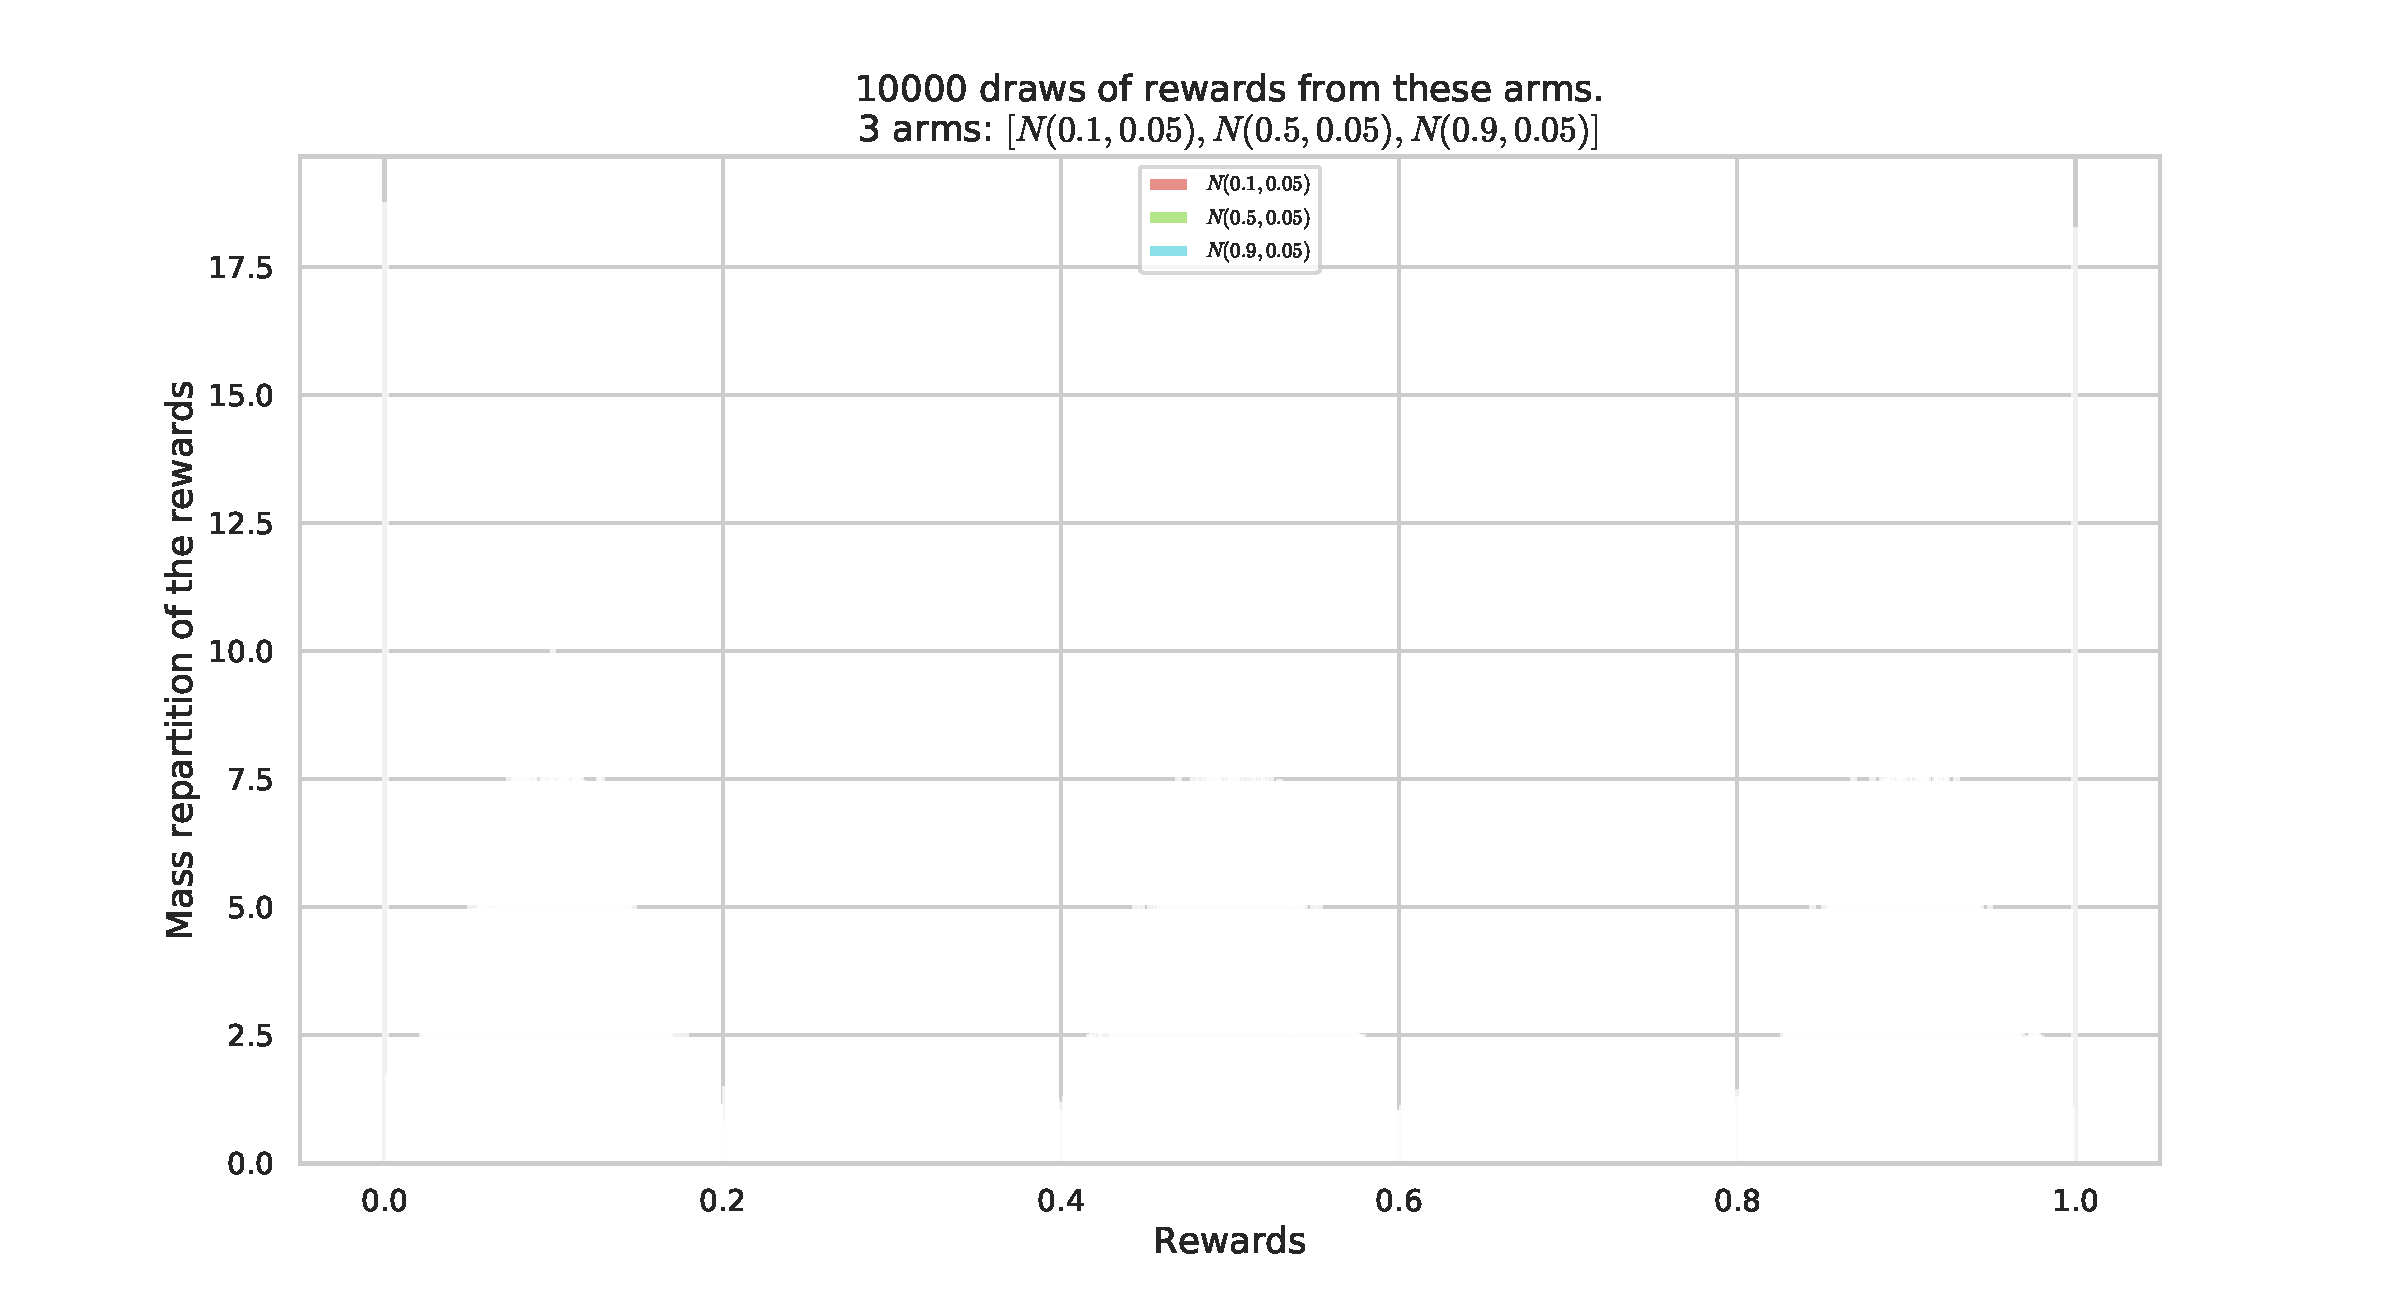
\includegraphics[width=0.75\linewidth]{exampleOfRewards.pdf}
	\caption{Histogram of $10000$ \iid{} rewards obtained from three arms with a Gaussian distribution truncated to $[0,1]$, of respective means $0.1$, $0.5$ and $0.9$.}
	\label{fig:3:exampleOfRewards}
\end{figure}


We do not give more details, but the interested reader can refer to the following Jupyter notebook \cite{jupyter} document hosted at:\\
\begin{small}
    \href{https://smpybandits.github.io/notebooks/Easily_creating_MAB_problems.html}{\texttt{SMPyBandits.GitHub.io/notebooks/Easily\_creating\_MAB\_problems.html}}
\end{small}

We have not yet tried to add support for higher dimensional distributions of rewards, \eg, linear bandit, but it would be an interesting extension of SMPyBandits.
%
However, note that our library does support finite-state real-valued Markov MAB models, where arms do not correspond to distributions but to Markov chains, in the two variants of \emph{rested} or \emph{restless} Markov chains, as introduced by \cite{Anantharam87b}.

\subsection{MAB algorithms}

SMPyBandits is a complete open-source implementation of single-player (classical) bandit algorithms,
containing over 65 (in the module \texttt{\href{https://SMPyBandits.GitHub.io/docs/Policies.html}{Policies}}) algorithms.
It uses a well-designed hierarchical structure and class inheritance scheme (as detailed on the various UML diagrams showed on the \texttt{\href{https://SMPyBandits.GitHub.io/uml_diagrams/README.html}{uml\_diagrams}} folder) to minimize redundancy in the codebase.
For instance, most existing algorithms are index-based, and new ones can be written easily by inheriting from the \texttt{IndexPolicy} class (\texttt{\href{https://SMPyBandits.GitHub.io/docs/Policies.IndexPolicy.html}{Policies.IndexPolicy}}).
An index-based algorithm computes an index $I_k(t)\in\mathbb{R}$ for each arm $k$ at time $t$ and simply play $A(t) = \arg\max_k I_k(t)$.
For instance the code specific to the UCB algorithm \cite{LaiRobbins85,Auer02} is as short as this (and fully documented):

% https://tex.stackexchange.com/a/12430/
\begin{small}
% \begin{listing}[h!]
    \inputminted[linenos=true,numbersep=5pt,frame=lines,framesep=2mm]{python3}{2-Chapters/3-Chapter/src/example_of_a_IndexPolicy_UCB.py}
    % \caption{Small snippet of code defining the UCB algorithm, as a simple example of an Index Policy}
    \captionof{listing}{Small snippet of code defining the UCB algorithm, as a simple example of an Index Policy \label{lst:3:smallIndexPolicy}.}
    % \label{lst:3:smallIndexPolicy}
% \end{listing}
\end{small}


\subsection{Features}

With this numerical framework, simulations can run on a single CPU or a multi-core machine using joblib \cite{joblib} (see Appendix~\ref{sub:3:parallelSimulations}),
and summary plots are automatically saved as high-quality PNG, PDF and EPS, using matplotlib \cite{matplotlib} and seaborn \cite{seaborn}.
Raw data from each simulation is also saved in a HDF5 file using h5py \cite{h5py}, an efficient and compressed binary format, to allow easy post-mortem exploration of simulation results.
Making new simulations is very easy, one only needs to write a configuration script (\texttt{configuration.py}), without needing a complete knowledge of the internal code architecture.

A complete Sphinx documentation, for each algorithm and all parts of the codebase, even including the constants in the different configuration files, is available here:
\texttt{\href{https://SMPyBandits.GitHub.io}{SMPyBandits.GitHub.io}}.


\subsection{How to run experiments?}

We show how to install SMPyBandits, and an example of how to run a simple experiment.
This bash snippet\footnote{~See this page \texttt{\href{https://SMPyBandits.GitHub.io/How_to_run_the_code.html}{SMPyBandits.GitHub.io/How\_to\_run\_the\_code.html}} for more details.} shows how to clone the code\footnote{~SMPyBandits is also available on Pypi, see \texttt{\href{https://pypi.org/project/SMPyBandits/}{pypi.org/project/SMPyBandits}}. You can install it directly with \texttt{sudo pip install SMPyBandits}, or from a \texttt{virtualenv} \cite{virtualenv}.},
and install the requirements for Python 3 (once):

% https://tex.stackexchange.com/a/12430/
\begin{small}
    \begin{listing}[h!]
        \begin{minted}[linenos=true,numbersep=5pt,frame=lines,framesep=2mm]{bash}
# 1. get the code in the folder you want
$ git clone https://GitHub.com/SMPyBandits/SMPyBandits.git
$ cd SMPyBandits.git
# 2. install the requirements
$ pip install -r requirements.txt
        \end{minted}
        \caption{Small snippet of Bash code to download and install dependencies of SMPyBandits.}
        % \captionof{listing}{Small snippet of Bash code to download and install dependencies of SMPyBandits \label{lst:3:howToInstallLibrary}.}
        \label{lst:3:howToInstallLibrary}
    \end{listing}
\end{small}

Launching simulations is easy, for instance this snippet shows how to start $N=1000$ repetitions of a simple non-Bayesian Bernoulli-distributed problem, for $K=9$ arms, an horizon of $T=10000$ and on $4$ CPUs.
It takes about $20$ minutes, on a standard $4$-cores $64$ bits GNU/Linux laptop.
Using environment variables (\texttt{N=1000} etc) in the command line is not required, but it is convenient:

% https://tex.stackexchange.com/a/12430/
\begin{small}
\begin{listing}[h!]
    \begin{minted}[linenos=true,numbersep=5pt,frame=lines,framesep=2mm]{bash}
# 3. run a single-player simulation
$ BAYES=False ARM_TYPE=Bernoulli N=1000 T=10000 K=9 N_JOBS=4 \
  MEANS=[0.1,0.2,0.3,0.4,0.5,0.6,0.7,0.8,0.9] \
  python3 main.py configuration.py
    \end{minted}
    \caption{Small snippet of Bash code to run a simple experiment with SMPyBandits.}
    % \captionof{listing}{Small snippet of Bash code to run a simple experiment with SMPyBandits \label{lst:3:howToRunBasicLibrary}.}
    \label{lst:3:howToRunBasicLibrary}
\end{listing}
\end{small}


\subsection{Example of a simulation and illustration}

A small script \texttt{configuration.py} (\texttt{\href{https://SMPyBandits.GitHub.io/docs/configuration.html}{SMPyBandits.GitHub.io/docs/configuration.html}}) is used to import the arm classes (\texttt{\href{https://SMPyBandits.GitHub.io/docs/Arms.html}{SMPyBandits.GitHub.io/docs/Arms.html}}), the policy classes (\texttt{\href{https://SMPyBandits.GitHub.io/docs/Policies.html}{SMPyBandits.GitHub.io/docs/Policies.html}}) and define the problems and the experiments.
Choosing the algorithms is easy by customizing the \texttt{configuration["policies"]} list in the \texttt{configuration.py} file.
For instance, one can compare the standard anytime \klUCB{} algorithm (class \texttt{\href{https://SMPyBandits.GitHub.io/docs/Policies.klUCB.html}{Policies.klUCB}}) against the non-anytime variant $\klUCB^{++}$ algorithm (\texttt{\href{https://SMPyBandits.GitHub.io/docs/Policies.klUCBPlusPlus.html}{Policies.klUCBPlusPlus}}), and also \UCB{} with $\alpha=1$ (\texttt{\href{https://SMPyBandits.GitHub.io/docs/Policies.UCBalpha.html}{Policies.UCB}}) and Thompson sampling (\texttt{\href{https://SMPyBandits.GitHub.io/docs/Policies.Thompson.html}{Policies.Thompson}}) with a Beta posterior (\texttt{\href{https://SMPyBandits.GitHub.io/docs/Policies.Posterior.Beta.html}{Policies.Posterior.Beta}})).

% https://tex.stackexchange.com/a/12430/
\begin{small}
\begin{listing}[h!]
    \begin{minted}[linenos=true,numbersep=5pt,frame=lines,framesep=2mm]{python3}
configuration["policies"] = [
  {"archtype": klUCB, "params": {"klucb": klucbBern}},
  {"archtype": klUCBPlusPlus, "params": {"horizon": T, "klucb": klucbBern}},
  {"archtype": UCBalpha, "params": {"alpha": 1}},
  {"archtype": Thompson, "params": {"posterior": Beta}}
]
    \end{minted}
    \caption{Small snippet of Python code to configure the list of algorithms tested on a problem.}
    % \captionof{listing}{Small snippet of Python code to configure the list of algorithms tested on a problem. \label{lst:3:howToConfigureAlgorithms}.}
    \label{lst:3:howToConfigureAlgorithms}
\end{listing}
\end{small}

\begin{figure}[h!]  % [htbp]
	% \centering
	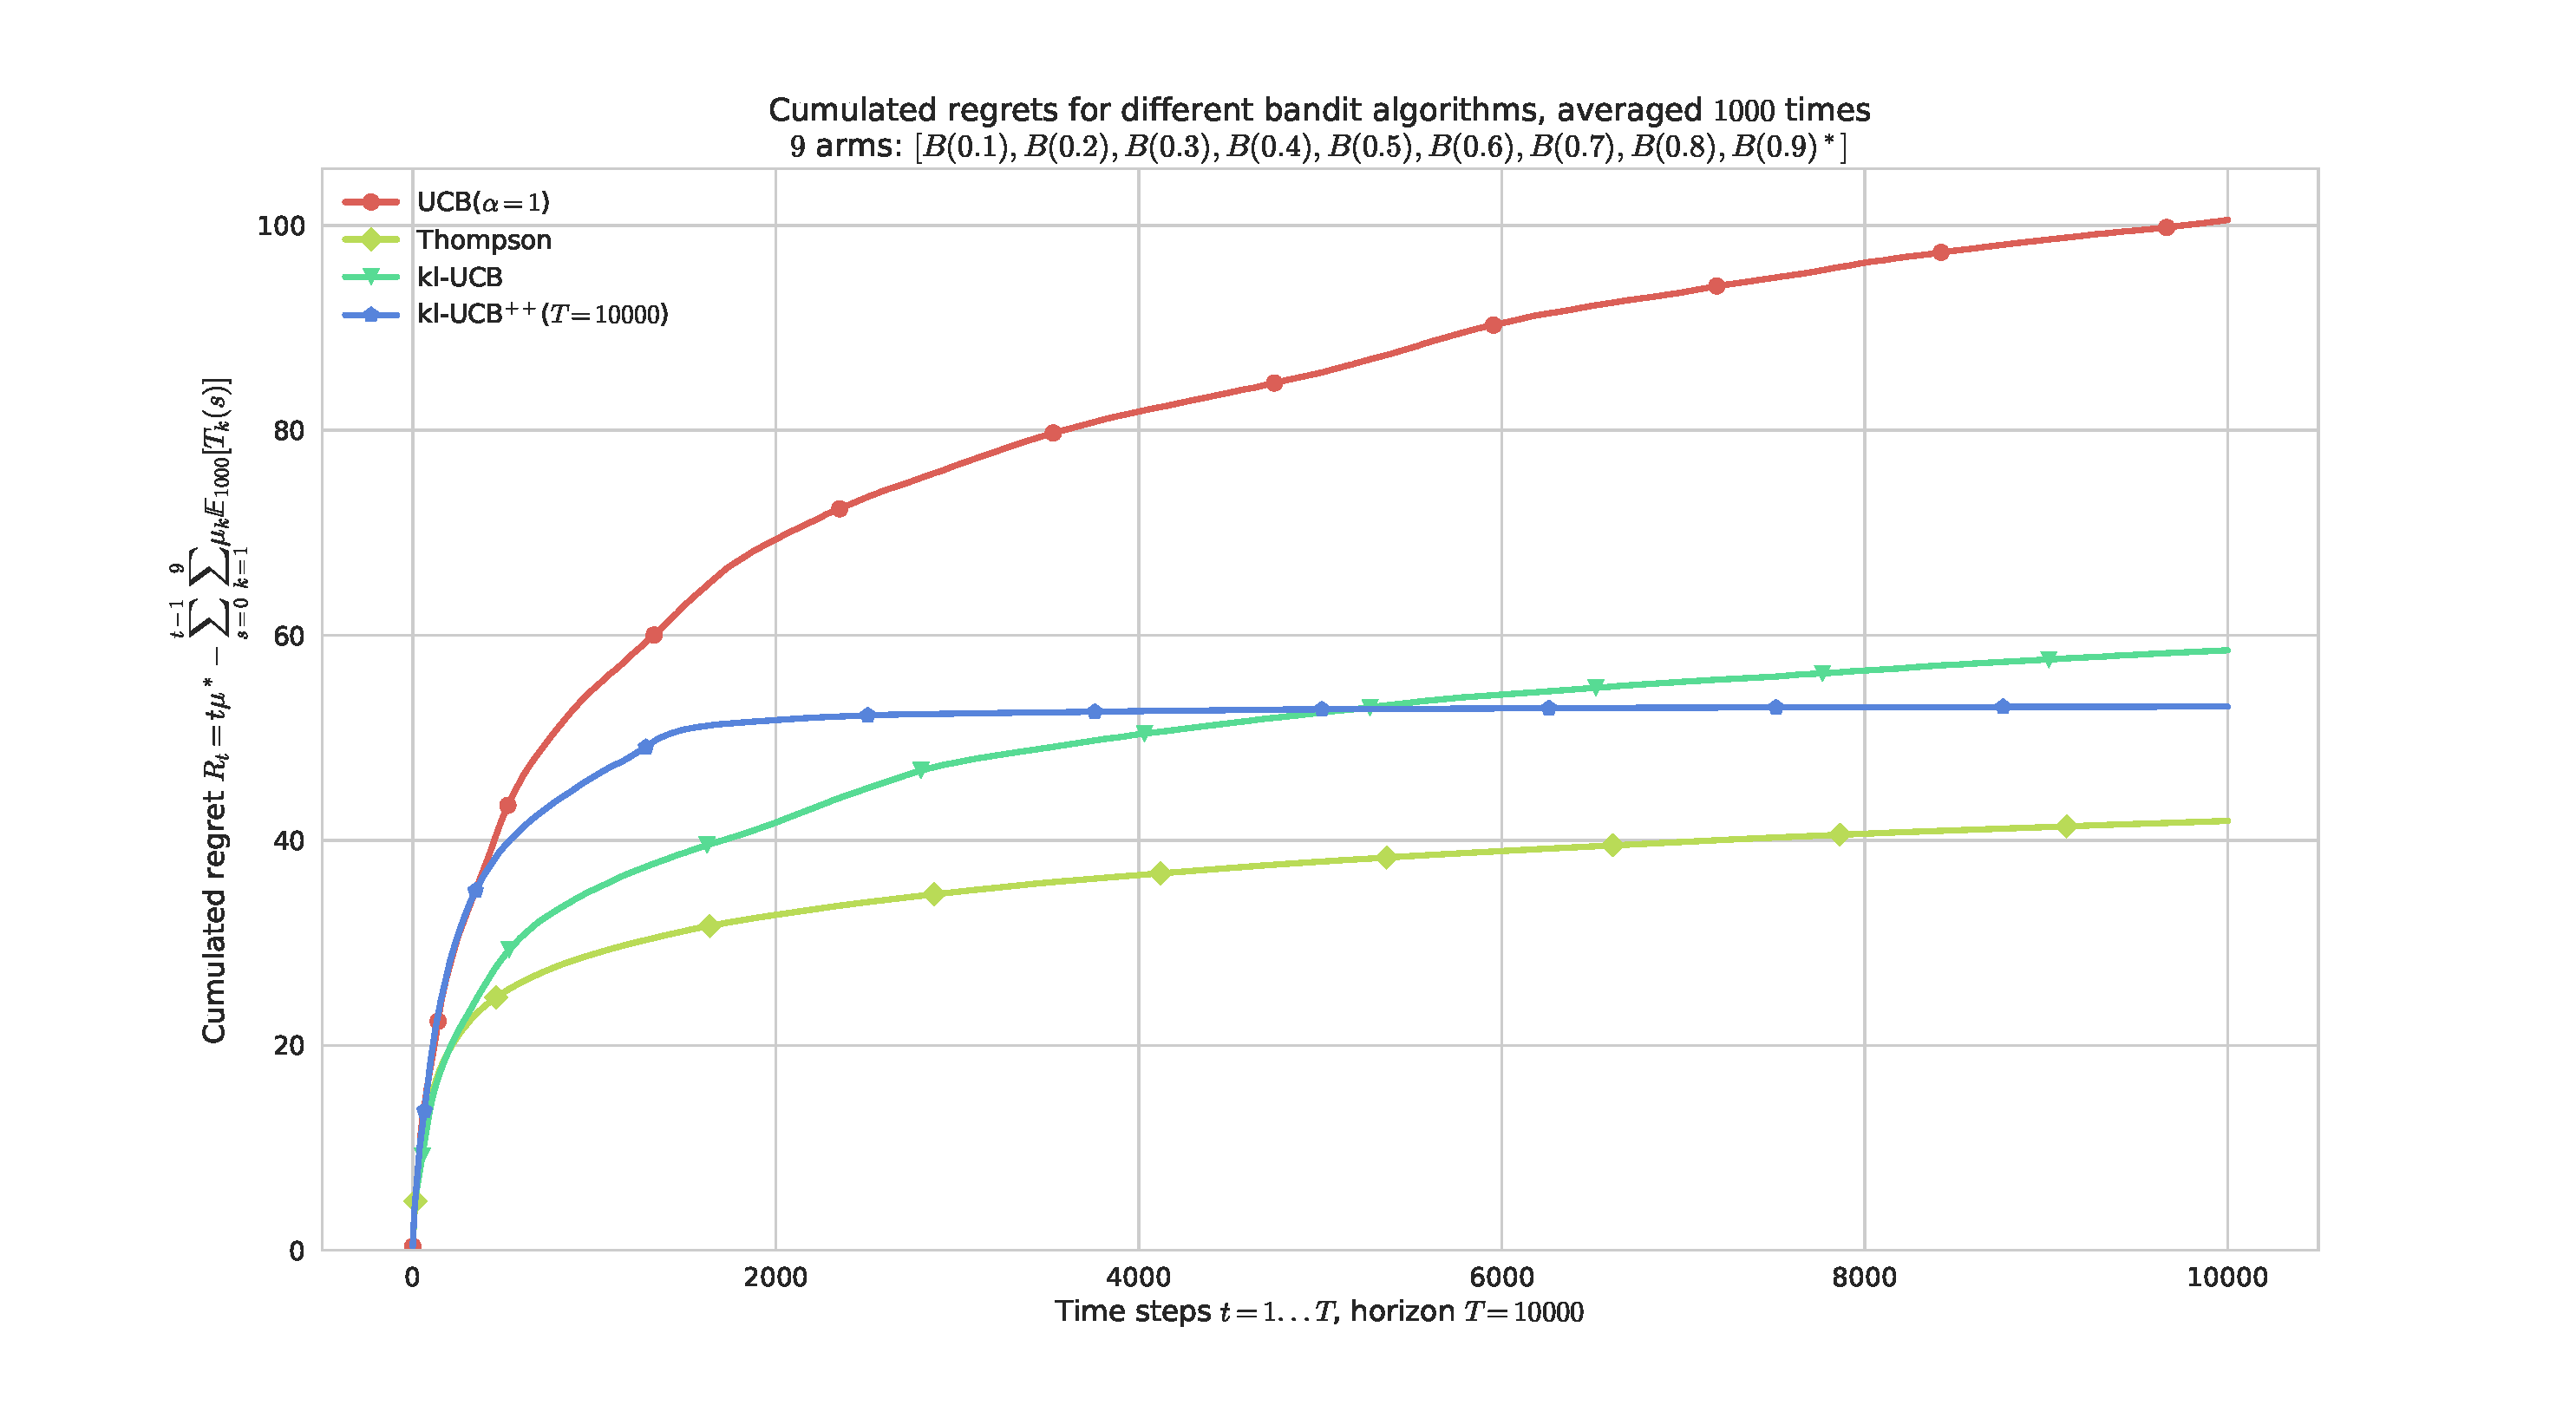
\includegraphics[width=1.05\linewidth]{3.pdf}
	\caption[Example of a single-player simulation showing the average regret and histogram of regrets of $4$ algorithms]{
		Example of a single-player simulation showing the average regret and histogram of regrets of four algorithms. They all perform very well: each algorithm is known to be order-optimal (\ie, its regret is proved to match the lower-bound up-to a constant), and each but UCB is known to be optimal (\ie, with the constant matching the lower-bound). For instance, Thomson sampling is very efficient in average (in yellow), and UCB shows a larger variance (in red).
	}
	\label{fig:3:firstPlot}
\end{figure}

Running the simulation as shown above will save figures in a sub-folder, as well as save data (pulls, rewards and regret) in a HDF5 file\footnote{~For example, this simulation produces this HDF5 file\\\texttt{\href{https://github.com/SMPyBandits/SMPyBandits/blob/master/plots/paper/example.hdf5}{GitHub.com/SMPyBandits/SMPyBandits/blob/master/plots/paper/example.hdf5}}}
\cite{h5py}.
% \texttt{\href{http://docs.h5py.org/en/stable/high/file.html}{docs.h5py.org/en/stable/high/file.html}}).
Figure~\ref{fig:3:firstPlot} above shows the average regret for these $4$ algorithms.
% The regret is the difference between the cumulated rewards of the best fixed-armed strategy (which is the oracle strategy for stationary bandits), and the cumulated rewards of the considered algorithms.
The Figure~\ref{fig:3:firstPlot_hist} below shows the histogram of regret obtained at the end of the experiment (\ie, $R_T$) for the same example.

\begin{figure}[h!]  % [htbp]
	% \centering
	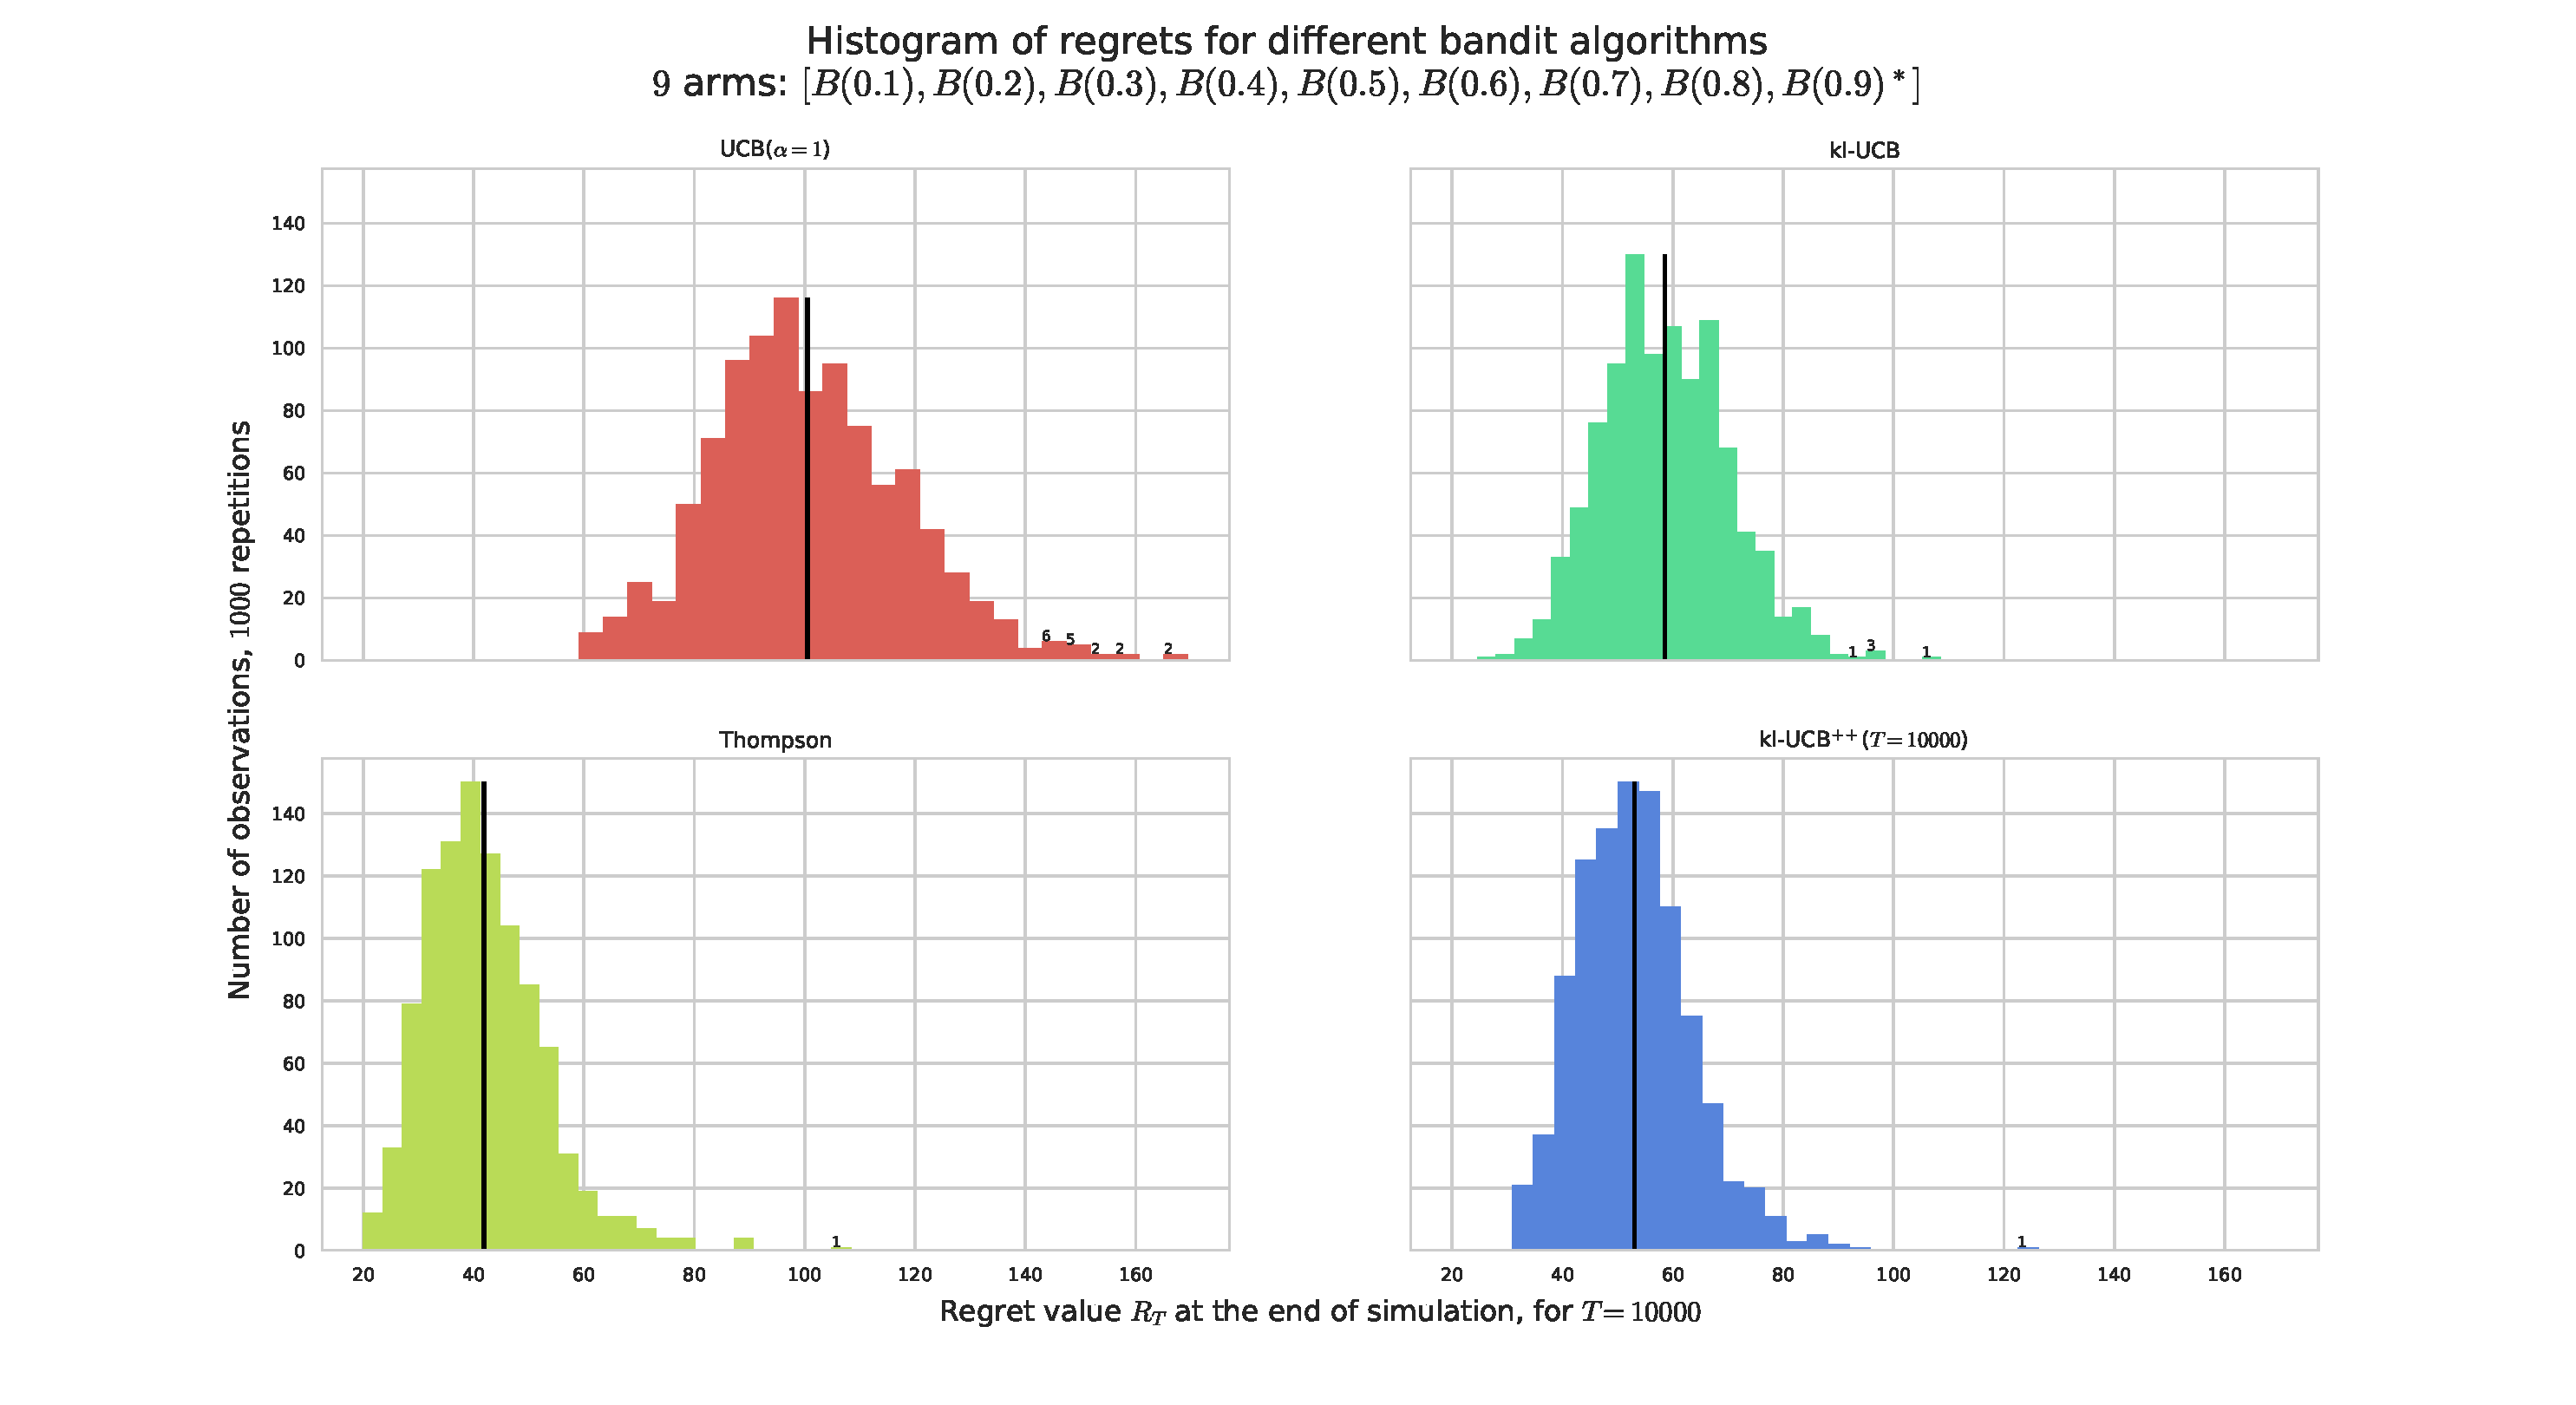
\includegraphics[width=1.05\linewidth]{3_hist.pdf}
	\caption{Histogram of regret for the same experiment.}
	\label{fig:3:firstPlot_hist}
\end{figure}


\subsection{Dependencies}
\label{sub:3:dependencies}

This library is written in Python \cite{python}, for versions 2.7+ or 3.4+, using \texttt{matplotlib} \cite{matplotlib} for 2D plotting, \texttt{numpy} \cite{numpy} for data storing, random number generations and operations on arrays, \texttt{scipy} \cite{scipy} for statistical and special functions, and \texttt{seaborn} \cite{seaborn} for pretty plotting and colorblind-aware colormaps.

Optional dependencies include \texttt{joblib} \cite{joblib} for parallel simulations, \texttt{numba} \cite{numba} for automatic speed-up on small functions using a Just-in-Time compiler, \texttt{sphinx} \cite{sphinx} for generating the documentation, \texttt{virtualenv} \cite{virtualenv} for launching simulations in isolated environments, and \texttt{jupyter} \cite{jupyter} used with \texttt{ipython} \cite{ipython} to experiment with the code.

All the quoted libraries are free and open-source and can be installed in one command using the \texttt{pip} (\texttt{\href{https://pip.pypa.io/}{pip.PyPa.io}}) or \texttt{conda} (\texttt{\href{http://conda.anaconda.org/}{conda.anaconda.org}}) package manager.
%
When SMPyBandits is installed using \texttt{pip install SMPyBandits}, the dependencies are of course automatically installed if not already present.


\subsection{Continuous integration with Read the Docs and Travis CI}

% \TODOL{I need to quickly explain that SMPyBandits is using Read the Docs since $2017$ and Travis Ci since $2018$ to: }

Since $2017$ and $2018$, SMPyBandits is using two online continuous integration (CI) service, to automatically build and host the documentation, and to automatically test the library on some numerical simulations.
%
These CI services are free for open-source works, and are both triggered whenever a modification of the codebase is sent to the hosting platform (\ie, GitHub).

\paragraph{Read the Docs.}
Since $2017$, we have been using the free web service provided by Read the Docs (\href{https://readthedocs.org/}{\texttt{ReadTheDocs.org}}).
Read the Docs allows to automatically build the documentation after every commit. This allows to regularly check that the library is well formatted and can be imported correctly, as well as keeping the online documentation up-to-date.
Moreover, they offer to host the documentation online, at \href{https://smpybandits.rtfd.io/}{\texttt{SMPyBandits.ReadTheDocs.io}}.
For more details, see \href{https://readthedocs.org/projects/smpybandits/}{\texttt{https://ReadTheDocs.org/projects/SMPyBandits}}.
%
Since its first use, the service did about 180 builds, and about $10\%$ of them were useful to detect newly introduced issues or bugs in the code.
The build is configured using the \texttt{.readthedocs.yml} file in SMPyBandits main folder, and it builds the documentation in about two minutes.
I have also been building the documentation manually on a weekly basis, to also host it on \href{https://smpybandits.github.io/}{\texttt{SMPyBandits.GitHub.io}} thanks to GitHub pages.
In the last two years, the documentation saw about 8500 unique visits, while the GitHub project have been visited about 3500 unique visits.


\paragraph{Travis CI.}
Since $2018$, we have been using the free web service provided by Travis CI (\href{https://travis-ci.org/}{\texttt{Travis-CI.org}}).
Travis CI allows to automatically run short numerical simulations after every commit.
This allows to check that each modification on any part of the codebase does not break anything, as well as giving an up-to-date example of log files that shows online the results of different examples of experiments. The tests covers all the main models and almost all the algorithms implemented in SMPyBandits, and it has been proved very useful to quickly find and fix new bugs.
For more details, see \href{https://travis-ci.org/SMPyBandits/SMPyBandits}{\texttt{Travis-CI.org/SMPyBandits/SMPyBandits}}.
%
Since its first use, the service did about 160 builds, and about $30\%$ of them were useful to detect newly introduced issues or bugs in the code.
The build is configured using the \texttt{.travis.yml} file in SMPyBandits main folder, and it runs numerical experiments with a short horizon (\eg, $T=100$ or $T=1000$) and a small number of repetitions (\ie, $N=4$), but covering all the different models implemented by SMPyBandits (and even including some that are not covered in this chapter, like the Markov model, or the sparse multi-player model).
Builds typically run for $15$ minutes, and Travis CI have been proved to be very useful in our development process.



\subsection{Research works using SMPyBandits}

SMPyBandits was used for the following research articles since $2017$, and it is used for the previous and the next chapters of this thesis (except in Chapter~\ref{chapter:4}).

-- In \cite{Besson2018WCNC} and in Chapter~\ref{chapter:2} above, we used SMPyBandits to illustrate and compare different aggregation algorithms\footnote{~See the page \texttt{\href{https://SMPyBandits.GitHub.io/Aggregation.html}{SMPyBandits.GitHub.io/Aggregation.html}} on the documentation, which gives detailed instructions to reproduce the results presented in this research paper, details about the models and the notations, and bibliographic references.}. We designed a variant of the Exp4 algorithm for online aggregation of experts \cite{Bubeck12}, called \texttt{\href{https://SMPyBandits.GitHub.io/docs/Policies.Aggregator.html}{Aggregator}}.
% Aggregating experts is a well-studied idea in sequential learning and in machine learning in general. We showed that it can be used in practice to select on the run the best bandit algorithm for a certain problem from a fixed pool of experts. This idea and algorithm can have interesting impact for Opportunistic Spectrum Access applications \cite{Jouini09} that use multi-armed bandits algorithms for sequential learning and network efficiency optimization.

-- In \cite{Besson2018ALT} and in Chapter~\ref{chapter:5} below, we used SMPyBandits for all the simulations for multi-player bandit algorithms\footnote{~Similarly, see the page \texttt{\href{https://SMPyBandits.GitHub.io/MultiPlayers.html}{SMPyBandits.GitHub.io/MultiPlayers.html}} on the documentation.}. We designed the two \texttt{\href{https://SMPyBandits.GitHub.io/docs/PoliciesMultiPlayers.RandTopM.html}{RandTopM}} and \texttt{\href{https://SMPyBandits.GitHub.io/docs/PoliciesMultiPlayers.MCTopM.html}{MCTopM}} algorithms and proved than they enjoy logarithmic regret in the usual setting, and outperform significantly the previous state-of-the-art solutions (\ie, \texttt{\href{https://SMPyBandits.GitHub.io/docs/PoliciesMultiPlayers.rhoRand.html}{rhoRand}}, \texttt{\href{https://SMPyBandits.GitHub.io/docs/Policies.MEGA.html}{MEGA}} and \texttt{\href{https://SMPyBandits.GitHub.io/docs/Policies.MusicalChair.html}{MusicalChair}}).

-- In \cite{Besson2018DoublingTricks} (quickly presented in Appendix~\ref{app:2:DoublingTricks}), we used SMPyBandits to illustrate and compare different "doubling trick" schemes\footnote{~Similarly, see the page \texttt{\href{https://SMPyBandits.GitHub.io/DoublingTrick.html}{SMPyBandits.GitHub.io/DoublingTrick.html}} on the documentation.}. and lots of bibliographic referencesIn sequential learning, an algorithm is anytime if it does not need to know the horizon $T$ of the experiments. A well-known trick for transforming any non-anytime algorithm to an anytime variant is the ``Doubling Trick'': start with an horizon $T_0\in\mathbb{N}^*$, and when $t > T_i$, use $T_{i+1} = 2 T_i$. We studied two generic sequences of growing horizons (geometric and exponential), and we proved two theorems that generalized previous results. A geometric sequence suffices to conserve minimax regret bounds (in $R_T = \mathcal{O}(\sqrt{T})$), with a constant multiplicative loss $\ell \leq 4$, but cannot be used to conserve a logarithmic regret bound (in $R_T = \mathcal{O}(\log(T))$). And an exponential sequence can be used to conserve logarithmic bounds, with a constant multiplicative loss also $\ell \leq 4$ in the usual setting. It is still an open question to know if a well-tuned exponential sequence can conserve minimax bounds, or "weak" minimax bounds (in $R_T = \mathcal{O}(\sqrt{T \log(T)})$).

-- In \cite{Besson2019GLRT} and \cite{Besson2019Gretsi}, and in Chapter~\ref{chapter:6} below, we used SMPyBandits for piece-wise stationary MAB models (only for the single-player case). We illustrate and compare different algorithms designed for this family of non-stationary problems\footnote{~Similarly, see the page \texttt{\href{https://SMPyBandits.GitHub.io/NonStationary.html}{SMPyBandits.GitHub.io/NonStationary.html}} on the documentation.}.
We designed the \texttt{\href{https://SMPyBandits.GitHub.io/docs/Policies.GLR_UCB.html}{GLRklUCB}} policy, and implemented most of the policies from state-of-the-art research on passively or active adaptive policies, both adversarial- or stochastic-based, designed to tackle the piece-wise stationary MAB problems.
We also implemented a large benchmark of different problems.


% ----------------------------------------------------------------------------
\section{Experimental comparisons of state-of-the-art single-player algorithms}
\label{sec:3:reviewSPAlgorithms}

\TODOL{Write text for this Section, write configuration.py file, run short-term experiment, include them, if happy about it, run longer ang larger experiments}

In this section, we use the SMPyBandits library to compare experimentally various state-of-the-art single-player algorithms on different kinds of multi-armed bandit problems.
First, we detail the list of different algorithms that we compare, and the different problems on which they are all tested.
We give the results of the numerical experiments, in terms of mean regret at the end of the experiment of different horizons $T$.
Additional results in terms of real measurements of time and memory are given and discussed in the next Section~\ref{sec:3:timeAndMemoryCosts}.

Finally, we give some observations on the results, and the main take-away message of this section is the following: in all the rest of this thesis, we focus on using the simple \UCB{} algorithm when simplicity is favored, \ie, in the more applied Chapter~\ref{chapter:4}, and the \klUCB{} algorithm when efficiency is favored, \ie, in the two more theoretical Chapters~\ref{chapter:5} and \ref{chapter:6}.


\subsection{Experimental setup: algorithms and problems}

\paragraph{List of algorithms}

We consider the nine following algorithms. For each of them, we give a bibliographic reference, that corresponds to the most recent article studying it and not the first one which introduced it.
We give the chosen tuning of the parameters, for parametric algorithms.
Algorithms that are not anytime use the exact value of the horizon $T$, and when increasing values of $T$ are studied for the same problem, of course they use the correct successive values.
We also give the name of the corresponding class in the \texttt{Policies} module in SMPyBandits.

% FIXME order from oldest to most recent, and simplest to more complex

\begin{itemize}
    \item Algorithm 1 is
    an $\varepsilon$-greedy algorithm, as described in \cite{Bubeck12}, using $\varepsilon_t = \varepsilon_0 / t$, and $\varepsilon_0 = 0.1$ (chosen arbitrarily) (\texttt{EpsilonDecreasing}).

    \item Algorithm 2 is
    an Explore-then-Commit algorithm from \cite{GarivierETC2016}, that knows the horizon, and a lower-bound on the gap between arms (chosen arbitrarily as $\delta=0.01$, valid for all problems) (\texttt{ETC\_KnownGap}).

    \item Algorithm 3 is
    $\mathrm{Exp}3^{++}$ from \cite{Seldin17}, using $\alpha=3$ and $\beta=256$ as advised (\texttt{Exp3PlusPlus}).

    \item Algorithm 4 is
    $\UCB_1$ from \cite{Auer02}, using $\alpha=1$ (\texttt{UCB}).

    \item Algorithm 5 is
    \klUCB{} from \cite{KLUCBJournal}, using the Bernoulli KL divergence and the corresponding \klUCB{} indexes, implemented as \texttt{kullback.klucbBern} (\texttt{klUCB}).

    \item Algorithm 6 is
    Thompson sampling from \cite{Kaufmann12Thompson}, using a Beta prior and posterior, initially uniform (\ie, $\mathrm{Beta}(1,1)$) (\texttt{Thompson}).

    \item Algorithm 7 is
    Bayes-UCB from \cite{Kaufmann12BUCB}, using a Beta prior and posterior, initially uniform (\ie, $\mathrm{Beta}(1,1)$) (\texttt{BayesUCB}).

    \item Algorithm 8 is
    AdBandits from \cite{Truzzi13}, using $\alpha=1$ (\texttt{AdBandits}).

    \item Algorithm 9 is
    BESA (Best Empirical Sampled Average) from \cite{Baransi2014}, using a binary tournament implement in a naive but efficient way (not using recursive functions) (\texttt{BESA} with \texttt{''non\_recursive''=True}).
\end{itemize}

In the results presented in the main text of this chapter, we focus on the most well known algorithms, and two others that are efficient but less known (AdBandits and BESA).
We present in Appendix~\ref{sub:3:additionalExperiments} seven other algorithms, being more recent (from $2016$, $3$ from $2018$ and $2$ from $2019$) but are usually more complex, or are based on a different point-of-view.
We include numerical results for these other algorithms as well, to justify empirically that despite their respective qualities, and despite being efficient, it is reasonable to focus on \UCB{} and \klUCB{} algorithms in the rest of this thesis.


\paragraph{Two different problems}

We consider two different problems, that are described here for a generic value of $K \geq 2$ the number of arms.
For simplicity, we focus on Bernoulli distributed arms, even if similar results were observed for other distributions, in particular for truncated or untruncated Gaussian distributions.

\begin{itemize}
    \item \textbf{Problem 1} considers $K$ arms of equally spaced means, in $[0,1]$.
    It uses a minimum mean of $0.05$ and a maximum mean of $0.95$.
    For instance, for $K=2$, $\bm{\mu}=[0.05, 0.95]$ and for $K=5$, $\bm{\mu} = [0.05, 0.275, 0.5, 0.725, 0.95]$.

    \item \textbf{Problem 2} takes another approach. Instead of simulating $1000$ times the same problem, it generates a new random problem for each independent run.
    It considers a randomly generated vector of means, each being sampled uniformly at random in $[0,1]$, with a minimum gap of $\Delta^{\min}$, $\bm{\mu} \sim \cE(\Delta^{\min},\mu_{\min},\mu_{\max})$, as well as minimum and maximum values of $\mu_{\min}$ and $\mu_{\max}$.
    This space $\cE_{\Delta^{\min}}$ is defined as $\{ \bm{\mu} \in [\mu_{\min}, \mu_{\max}]^K : \min_{k\neq k'} |\mu_k - \mu_{k'}| \geq \Delta^{\min} \}$.
    We use $\mu_{\min} = \Delta^{\min}$ and $\mu_{\max} = 1 - \Delta^{\min}$,
    and the value used for $\Delta^{\min}$ is $0.1$ for $K \leq 3$ (for ``easy'' problems), and $\frac{1}{3 K}$ for $K \geq 5$ (for ``harder'' problems).
    % 0.1 if NB_ARMS <= 5 else 1. / (3 * NB_ARMS)
\end{itemize}


\paragraph{Other parameters of the experiments}

We consider increasing values for the horizon, $T=1000$, $T=5000$, $T=10000$ and $T=50000$.  % FIXME update if needed?
We consider as well an increasing number of arms, $K=2$, $K=5$, $K=9$, $K=20$ and $K=50$.  % FIXME update if needed?
For all experiments, we run $N=1000$ independent simulations.  % FIXME update if needed?


\subsection{Experiments results}

We give in the tables below the results of the experiments. For the two different problems and different values of $T$ and $K$, we give the mean $\pm 1$ standard-variation of the empirical regret $R_T$ obtained by the different algorithms at the end of the experiments.
Tables~\ref{table:3:meanRegret_problem1} is for the fixed-gap \textbf{problem 1}
and \ref{table:3:meanRegret_problem2} is for the randomly generated \textbf{problem 2}.
Each column corresponds to one value of $T$, and each line corresponds to one algorithm.
For each cell, we report successive values that correspond to the successive values of the number of arms $K$.

\TODOL{FIXME launch these experiments, for a very short number of repetitions N=4, and if I'm happy about the results and if they are easily copied-and-pasted here, then launch with N=100 or N=1000 depending on the running time of the whole simulations}

% DEBUG=True; NOPLOTS=False; SAVEALL=False; for N in 4 100 1000; do for BAYES in False True; do for T in 1000 5000 10000 50000; do for K in 2 5 10 20 50; do debut=$(date); DEBUG=$DEBUG NOPLOTS=$NOPLOTS SAVEALL=$SAVEALL N=$N N_JOBS=-1 T=$T K=$K BAYES=$BAYES make --noFreeSMS single && cp logs/main_py3_log.txt logs/main_py3_log__N${N}_BAYES${BAYES}_T{T}_K{K}.txt && FreeSMS.py "Expérience commencée ${debut} terminée, avec N=${N}, BAYES=${BAYES}, T=${T}, K=${K}." ; done; done; done; done time.

\begin{table}[!t]
\begin{footnotesize}  % WARNING
    \centering
    \begin{tabular}{c|*{5}{m{2cm}}} % WARNING size ?
    \textbf{Algorithms} $\;$ \textbackslash $\;$ $\mathbf{T=}$
        & $T_1 = 1000$ & $T_2 = 5000$ & $T_3 = 10000$ & $T_4 = 50000$ \\
        \hline
        $\varepsilon$-greedy &
            $R^{1}_{T_1,K_1} = 0 \pm 0$
                $R^{1}_{T_1,K_2} = 0 \pm 0$
                $R^{1}_{T_1,K_3} = 0 \pm 0$
                $R^{1}_{T_1,K_4} = 0 \pm 0$
                $R^{1}_{T_1,K_5} = 0 \pm 0$ &
            $R^{1}_{T_2,K_1} = 0 \pm 0$
                $R^{1}_{T_2,K_2} = 0 \pm 0$
                $R^{1}_{T_2,K_3} = 0 \pm 0$
                $R^{1}_{T_2,K_4} = 0 \pm 0$
                $R^{1}_{T_2,K_5} = 0 \pm 0$ &
            $R^{1}_{T_3,K_1} = 0 \pm 0$
                $R^{1}_{T_3,K_2} = 0 \pm 0$
                $R^{1}_{T_3,K_3} = 0 \pm 0$
                $R^{1}_{T_3,K_4} = 0 \pm 0$
                $R^{1}_{T_3,K_5} = 0 \pm 0$ &
            $R^{1}_{T_4,K_1} = 0 \pm 0$
                $R^{1}_{T_4,K_2} = 0 \pm 0$
                $R^{1}_{T_4,K_3} = 0 \pm 0$
                $R^{1}_{T_4,K_4} = 0 \pm 0$
                $R^{1}_{T_4,K_5} = 0 \pm 0$ \\
        \hline
        Explore-then-Commit &
            $R^{2}_{T_1,K_1} = 0 \pm 0$
                $R^{2}_{T_1,K_2} = 0 \pm 0$
                $R^{2}_{T_1,K_3} = 0 \pm 0$
                $R^{2}_{T_1,K_4} = 0 \pm 0$
                $R^{2}_{T_1,K_5} = 0 \pm 0$ &
            $R^{2}_{T_2,K_1} = 0 \pm 0$
                $R^{2}_{T_2,K_2} = 0 \pm 0$
                $R^{2}_{T_2,K_3} = 0 \pm 0$
                $R^{2}_{T_2,K_4} = 0 \pm 0$
                $R^{2}_{T_2,K_5} = 0 \pm 0$ &
            $R^{2}_{T_3,K_1} = 0 \pm 0$
                $R^{2}_{T_3,K_2} = 0 \pm 0$
                $R^{2}_{T_3,K_3} = 0 \pm 0$
                $R^{2}_{T_3,K_4} = 0 \pm 0$
                $R^{2}_{T_3,K_5} = 0 \pm 0$ &
            $R^{2}_{T_4,K_1} = 0 \pm 0$
                $R^{2}_{T_4,K_2} = 0 \pm 0$
                $R^{2}_{T_4,K_3} = 0 \pm 0$
                $R^{2}_{T_4,K_4} = 0 \pm 0$
                $R^{2}_{T_4,K_5} = 0 \pm 0$ \\
        \hline
        $\mathrm{Exp}3^{++}$ &
            $R^3_{T_1,K_1} = 0 \pm 0$
                $R^3_{T_1,K_2} = 0 \pm 0$
                $R^3_{T_1,K_3} = 0 \pm 0$
                $R^3_{T_1,K_4} = 0 \pm 0$
                $R^3_{T_1,K_5} = 0 \pm 0$ &
            $R^3_{T_2,K_1} = 0 \pm 0$
                $R^3_{T_2,K_2} = 0 \pm 0$
                $R^3_{T_2,K_3} = 0 \pm 0$
                $R^3_{T_2,K_4} = 0 \pm 0$
                $R^3_{T_2,K_5} = 0 \pm 0$ &
            $R^3_{T_3,K_1} = 0 \pm 0$
                $R^3_{T_3,K_2} = 0 \pm 0$
                $R^3_{T_3,K_3} = 0 \pm 0$
                $R^3_{T_3,K_4} = 0 \pm 0$
                $R^3_{T_3,K_5} = 0 \pm 0$ &
            $R^3_{T_4,K_1} = 0 \pm 0$
                $R^3_{T_4,K_2} = 0 \pm 0$
                $R^3_{T_4,K_3} = 0 \pm 0$
                $R^3_{T_4,K_4} = 0 \pm 0$
                $R^3_{T_4,K_5} = 0 \pm 0$ \\
        \hline
        $\UCB_1$ &
            $R^{4}_{T_1,K_1} = 0 \pm 0$
                $R^{4}_{T_1,K_2} = 0 \pm 0$
                $R^{4}_{T_1,K_3} = 0 \pm 0$
                $R^{4}_{T_1,K_4} = 0 \pm 0$
                $R^{4}_{T_1,K_5} = 0 \pm 0$ &
            $R^{4}_{T_2,K_1} = 0 \pm 0$
                $R^{4}_{T_2,K_2} = 0 \pm 0$
                $R^{4}_{T_2,K_3} = 0 \pm 0$
                $R^{4}_{T_2,K_4} = 0 \pm 0$
                $R^{4}_{T_2,K_5} = 0 \pm 0$ &
            $R^{4}_{T_3,K_1} = 0 \pm 0$
                $R^{4}_{T_3,K_2} = 0 \pm 0$
                $R^{4}_{T_3,K_3} = 0 \pm 0$
                $R^{4}_{T_3,K_4} = 0 \pm 0$
                $R^{4}_{T_3,K_5} = 0 \pm 0$ &
            $R^{4}_{T_4,K_1} = 0 \pm 0$
                $R^{4}_{T_4,K_2} = 0 \pm 0$
                $R^{4}_{T_4,K_3} = 0 \pm 0$
                $R^{4}_{T_4,K_4} = 0 \pm 0$
                $R^{4}_{T_4,K_5} = 0 \pm 0$ \\
        \hline
        \klUCB{} &
            $R^{5}_{T_1,K_1} = 0 \pm 0$
                $R^{5}_{T_1,K_2} = 0 \pm 0$
                $R^{5}_{T_1,K_3} = 0 \pm 0$
                $R^{5}_{T_1,K_4} = 0 \pm 0$
                $R^{5}_{T_1,K_5} = 0 \pm 0$ &
            $R^{5}_{T_2,K_1} = 0 \pm 0$
                $R^{5}_{T_2,K_2} = 0 \pm 0$
                $R^{5}_{T_2,K_3} = 0 \pm 0$
                $R^{5}_{T_2,K_4} = 0 \pm 0$
                $R^{5}_{T_2,K_5} = 0 \pm 0$ &
            $R^{5}_{T_3,K_1} = 0 \pm 0$
                $R^{5}_{T_3,K_2} = 0 \pm 0$
                $R^{5}_{T_3,K_3} = 0 \pm 0$
                $R^{5}_{T_3,K_4} = 0 \pm 0$
                $R^{5}_{T_3,K_5} = 0 \pm 0$ &
            $R^{5}_{T_4,K_1} = 0 \pm 0$
                $R^{5}_{T_4,K_2} = 0 \pm 0$
                $R^{5}_{T_4,K_3} = 0 \pm 0$
                $R^{5}_{T_4,K_4} = 0 \pm 0$
                $R^{5}_{T_4,K_5} = 0 \pm 0$ \\
        \hline
        Thompson sampling &
            $R^{6}_{T_1,K_1} = 0 \pm 0$
                $R^{6}_{T_1,K_2} = 0 \pm 0$
                $R^{6}_{T_1,K_3} = 0 \pm 0$
                $R^{6}_{T_1,K_4} = 0 \pm 0$
                $R^{6}_{T_1,K_5} = 0 \pm 0$ &
            $R^{6}_{T_2,K_1} = 0 \pm 0$
                $R^{6}_{T_2,K_2} = 0 \pm 0$
                $R^{6}_{T_2,K_3} = 0 \pm 0$
                $R^{6}_{T_2,K_4} = 0 \pm 0$
                $R^{6}_{T_2,K_5} = 0 \pm 0$ &
            $R^{6}_{T_3,K_1} = 0 \pm 0$
                $R^{6}_{T_3,K_2} = 0 \pm 0$
                $R^{6}_{T_3,K_3} = 0 \pm 0$
                $R^{6}_{T_3,K_4} = 0 \pm 0$
                $R^{6}_{T_3,K_5} = 0 \pm 0$ &
            $R^{6}_{T_4,K_1} = 0 \pm 0$
                $R^{6}_{T_4,K_2} = 0 \pm 0$
                $R^{6}_{T_4,K_3} = 0 \pm 0$
                $R^{6}_{T_4,K_4} = 0 \pm 0$
                $R^{6}_{T_4,K_5} = 0 \pm 0$ \\
        \hline
        Thompson sampling &
            $R^{7}_{T_1,K_1} = 0 \pm 0$
                $R^{7}_{T_1,K_2} = 0 \pm 0$
                $R^{7}_{T_1,K_3} = 0 \pm 0$
                $R^{7}_{T_1,K_4} = 0 \pm 0$
                $R^{7}_{T_1,K_5} = 0 \pm 0$ &
            $R^{7}_{T_2,K_1} = 0 \pm 0$
                $R^{7}_{T_2,K_2} = 0 \pm 0$
                $R^{7}_{T_2,K_3} = 0 \pm 0$
                $R^{7}_{T_2,K_4} = 0 \pm 0$
                $R^{7}_{T_2,K_5} = 0 \pm 0$ &
            $R^{7}_{T_3,K_1} = 0 \pm 0$
                $R^{7}_{T_3,K_2} = 0 \pm 0$
                $R^{7}_{T_3,K_3} = 0 \pm 0$
                $R^{7}_{T_3,K_4} = 0 \pm 0$
                $R^{7}_{T_3,K_5} = 0 \pm 0$ &
            $R^{7}_{T_4,K_1} = 0 \pm 0$
                $R^{7}_{T_4,K_2} = 0 \pm 0$
                $R^{7}_{T_4,K_3} = 0 \pm 0$
                $R^{7}_{T_4,K_4} = 0 \pm 0$
                $R^{7}_{T_4,K_5} = 0 \pm 0$ \\
        \hline
        AdBandits &
            $R^{8}_{T_1,K_1} = 0 \pm 0$
                $R^{8}_{T_1,K_2} = 0 \pm 0$
                $R^{8}_{T_1,K_3} = 0 \pm 0$
                $R^{8}_{T_1,K_4} = 0 \pm 0$
                $R^{8}_{T_1,K_5} = 0 \pm 0$ &
            $R^{8}_{T_2,K_1} = 0 \pm 0$
                $R^{8}_{T_2,K_2} = 0 \pm 0$
                $R^{8}_{T_2,K_3} = 0 \pm 0$
                $R^{8}_{T_2,K_4} = 0 \pm 0$
                $R^{8}_{T_2,K_5} = 0 \pm 0$ &
            $R^{8}_{T_3,K_1} = 0 \pm 0$
                $R^{8}_{T_3,K_2} = 0 \pm 0$
                $R^{8}_{T_3,K_3} = 0 \pm 0$
                $R^{8}_{T_3,K_4} = 0 \pm 0$
                $R^{8}_{T_3,K_5} = 0 \pm 0$ &
            $R^{8}_{T_4,K_1} = 0 \pm 0$
                $R^{8}_{T_4,K_2} = 0 \pm 0$
                $R^{8}_{T_4,K_3} = 0 \pm 0$
                $R^{8}_{T_4,K_4} = 0 \pm 0$
                $R^{8}_{T_4,K_5} = 0 \pm 0$ \\
        \hline
        BESA &
            $R^{9}_{T_1,K_1} = 0 \pm 0$
                $R^{9}_{T_1,K_2} = 0 \pm 0$
                $R^{9}_{T_1,K_3} = 0 \pm 0$
                $R^{9}_{T_1,K_4} = 0 \pm 0$
                $R^{9}_{T_1,K_5} = 0 \pm 0$ &
            $R^{9}_{T_2,K_1} = 0 \pm 0$
                $R^{9}_{T_2,K_2} = 0 \pm 0$
                $R^{9}_{T_2,K_3} = 0 \pm 0$
                $R^{9}_{T_2,K_4} = 0 \pm 0$
                $R^{9}_{T_2,K_5} = 0 \pm 0$ &
            $R^{9}_{T_3,K_1} = 0 \pm 0$
                $R^{9}_{T_3,K_2} = 0 \pm 0$
                $R^{9}_{T_3,K_3} = 0 \pm 0$
                $R^{9}_{T_3,K_4} = 0 \pm 0$
                $R^{9}_{T_3,K_5} = 0 \pm 0$ &
            $R^{9}_{T_4,K_1} = 0 \pm 0$
                $R^{9}_{T_4,K_2} = 0 \pm 0$
                $R^{9}_{T_4,K_3} = 0 \pm 0$
                $R^{9}_{T_4,K_4} = 0 \pm 0$
                $R^{9}_{T_4,K_5} = 0 \pm 0$ \\
        \hline
    \end{tabular}
    \caption{Mean regret $\pm$ $1$ std-dev, for $9$ different algorithms on \textbf{problem 1} with different values of time $T$ and number of arm $K$.
    }
    \label{table:3:meanRegret_problem1}
\end{footnotesize}  % WARNING
\end{table}


\begin{table}[!t]
\begin{footnotesize}  % WARNING
    \centering
    \begin{tabular}{c|*{5}{m{2cm}}} % WARNING size ?
    \textbf{Algorithms} $\;$ \textbackslash $\;$ $\mathbf{T=}$
        & $T_1 = 1000$ & $T_2 = 5000$ & $T_3 = 10000$ & $T_4 = 50000$ \\
        \hline
        $\varepsilon$-greedy &
            $R^{1}_{T_1,K_1} = 0 \pm 0$
                $R^{1}_{T_1,K_2} = 0 \pm 0$
                $R^{1}_{T_1,K_3} = 0 \pm 0$
                $R^{1}_{T_1,K_4} = 0 \pm 0$
                $R^{1}_{T_1,K_5} = 0 \pm 0$ &
            $R^{1}_{T_2,K_1} = 0 \pm 0$
                $R^{1}_{T_2,K_2} = 0 \pm 0$
                $R^{1}_{T_2,K_3} = 0 \pm 0$
                $R^{1}_{T_2,K_4} = 0 \pm 0$
                $R^{1}_{T_2,K_5} = 0 \pm 0$ &
            $R^{1}_{T_3,K_1} = 0 \pm 0$
                $R^{1}_{T_3,K_2} = 0 \pm 0$
                $R^{1}_{T_3,K_3} = 0 \pm 0$
                $R^{1}_{T_3,K_4} = 0 \pm 0$
                $R^{1}_{T_3,K_5} = 0 \pm 0$ &
            $R^{1}_{T_4,K_1} = 0 \pm 0$
                $R^{1}_{T_4,K_2} = 0 \pm 0$
                $R^{1}_{T_4,K_3} = 0 \pm 0$
                $R^{1}_{T_4,K_4} = 0 \pm 0$
                $R^{1}_{T_4,K_5} = 0 \pm 0$ \\
        \hline
        Explore-then-Commit &
            $R^{2}_{T_1,K_1} = 0 \pm 0$
                $R^{2}_{T_1,K_2} = 0 \pm 0$
                $R^{2}_{T_1,K_3} = 0 \pm 0$
                $R^{2}_{T_1,K_4} = 0 \pm 0$
                $R^{2}_{T_1,K_5} = 0 \pm 0$ &
            $R^{2}_{T_2,K_1} = 0 \pm 0$
                $R^{2}_{T_2,K_2} = 0 \pm 0$
                $R^{2}_{T_2,K_3} = 0 \pm 0$
                $R^{2}_{T_2,K_4} = 0 \pm 0$
                $R^{2}_{T_2,K_5} = 0 \pm 0$ &
            $R^{2}_{T_3,K_1} = 0 \pm 0$
                $R^{2}_{T_3,K_2} = 0 \pm 0$
                $R^{2}_{T_3,K_3} = 0 \pm 0$
                $R^{2}_{T_3,K_4} = 0 \pm 0$
                $R^{2}_{T_3,K_5} = 0 \pm 0$ &
            $R^{2}_{T_4,K_1} = 0 \pm 0$
                $R^{2}_{T_4,K_2} = 0 \pm 0$
                $R^{2}_{T_4,K_3} = 0 \pm 0$
                $R^{2}_{T_4,K_4} = 0 \pm 0$
                $R^{2}_{T_4,K_5} = 0 \pm 0$ \\
        \hline
        $\mathrm{Exp}3^{++}$ &
            $R^3_{T_1,K_1} = 0 \pm 0$
                $R^3_{T_1,K_2} = 0 \pm 0$
                $R^3_{T_1,K_3} = 0 \pm 0$
                $R^3_{T_1,K_4} = 0 \pm 0$
                $R^3_{T_1,K_5} = 0 \pm 0$ &
            $R^3_{T_2,K_1} = 0 \pm 0$
                $R^3_{T_2,K_2} = 0 \pm 0$
                $R^3_{T_2,K_3} = 0 \pm 0$
                $R^3_{T_2,K_4} = 0 \pm 0$
                $R^3_{T_2,K_5} = 0 \pm 0$ &
            $R^3_{T_3,K_1} = 0 \pm 0$
                $R^3_{T_3,K_2} = 0 \pm 0$
                $R^3_{T_3,K_3} = 0 \pm 0$
                $R^3_{T_3,K_4} = 0 \pm 0$
                $R^3_{T_3,K_5} = 0 \pm 0$ &
            $R^3_{T_4,K_1} = 0 \pm 0$
                $R^3_{T_4,K_2} = 0 \pm 0$
                $R^3_{T_4,K_3} = 0 \pm 0$
                $R^3_{T_4,K_4} = 0 \pm 0$
                $R^3_{T_4,K_5} = 0 \pm 0$ \\
        \hline
        $\UCB_1$ &
            $R^{4}_{T_1,K_1} = 0 \pm 0$
                $R^{4}_{T_1,K_2} = 0 \pm 0$
                $R^{4}_{T_1,K_3} = 0 \pm 0$
                $R^{4}_{T_1,K_4} = 0 \pm 0$
                $R^{4}_{T_1,K_5} = 0 \pm 0$ &
            $R^{4}_{T_2,K_1} = 0 \pm 0$
                $R^{4}_{T_2,K_2} = 0 \pm 0$
                $R^{4}_{T_2,K_3} = 0 \pm 0$
                $R^{4}_{T_2,K_4} = 0 \pm 0$
                $R^{4}_{T_2,K_5} = 0 \pm 0$ &
            $R^{4}_{T_3,K_1} = 0 \pm 0$
                $R^{4}_{T_3,K_2} = 0 \pm 0$
                $R^{4}_{T_3,K_3} = 0 \pm 0$
                $R^{4}_{T_3,K_4} = 0 \pm 0$
                $R^{4}_{T_3,K_5} = 0 \pm 0$ &
            $R^{4}_{T_4,K_1} = 0 \pm 0$
                $R^{4}_{T_4,K_2} = 0 \pm 0$
                $R^{4}_{T_4,K_3} = 0 \pm 0$
                $R^{4}_{T_4,K_4} = 0 \pm 0$
                $R^{4}_{T_4,K_5} = 0 \pm 0$ \\
        \hline
        \klUCB{} &
            $R^{5}_{T_1,K_1} = 0 \pm 0$
                $R^{5}_{T_1,K_2} = 0 \pm 0$
                $R^{5}_{T_1,K_3} = 0 \pm 0$
                $R^{5}_{T_1,K_4} = 0 \pm 0$
                $R^{5}_{T_1,K_5} = 0 \pm 0$ &
            $R^{5}_{T_2,K_1} = 0 \pm 0$
                $R^{5}_{T_2,K_2} = 0 \pm 0$
                $R^{5}_{T_2,K_3} = 0 \pm 0$
                $R^{5}_{T_2,K_4} = 0 \pm 0$
                $R^{5}_{T_2,K_5} = 0 \pm 0$ &
            $R^{5}_{T_3,K_1} = 0 \pm 0$
                $R^{5}_{T_3,K_2} = 0 \pm 0$
                $R^{5}_{T_3,K_3} = 0 \pm 0$
                $R^{5}_{T_3,K_4} = 0 \pm 0$
                $R^{5}_{T_3,K_5} = 0 \pm 0$ &
            $R^{5}_{T_4,K_1} = 0 \pm 0$
                $R^{5}_{T_4,K_2} = 0 \pm 0$
                $R^{5}_{T_4,K_3} = 0 \pm 0$
                $R^{5}_{T_4,K_4} = 0 \pm 0$
                $R^{5}_{T_4,K_5} = 0 \pm 0$ \\
        \hline
        Thompson sampling &
            $R^{6}_{T_1,K_1} = 0 \pm 0$
                $R^{6}_{T_1,K_2} = 0 \pm 0$
                $R^{6}_{T_1,K_3} = 0 \pm 0$
                $R^{6}_{T_1,K_4} = 0 \pm 0$
                $R^{6}_{T_1,K_5} = 0 \pm 0$ &
            $R^{6}_{T_2,K_1} = 0 \pm 0$
                $R^{6}_{T_2,K_2} = 0 \pm 0$
                $R^{6}_{T_2,K_3} = 0 \pm 0$
                $R^{6}_{T_2,K_4} = 0 \pm 0$
                $R^{6}_{T_2,K_5} = 0 \pm 0$ &
            $R^{6}_{T_3,K_1} = 0 \pm 0$
                $R^{6}_{T_3,K_2} = 0 \pm 0$
                $R^{6}_{T_3,K_3} = 0 \pm 0$
                $R^{6}_{T_3,K_4} = 0 \pm 0$
                $R^{6}_{T_3,K_5} = 0 \pm 0$ &
            $R^{6}_{T_4,K_1} = 0 \pm 0$
                $R^{6}_{T_4,K_2} = 0 \pm 0$
                $R^{6}_{T_4,K_3} = 0 \pm 0$
                $R^{6}_{T_4,K_4} = 0 \pm 0$
                $R^{6}_{T_4,K_5} = 0 \pm 0$ \\
        \hline
        Bayes-UCB &
            $R^{7}_{T_1,K_1} = 0 \pm 0$
                $R^{7}_{T_1,K_2} = 0 \pm 0$
                $R^{7}_{T_1,K_3} = 0 \pm 0$
                $R^{7}_{T_1,K_4} = 0 \pm 0$
                $R^{7}_{T_1,K_5} = 0 \pm 0$ &
            $R^{7}_{T_2,K_1} = 0 \pm 0$
                $R^{7}_{T_2,K_2} = 0 \pm 0$
                $R^{7}_{T_2,K_3} = 0 \pm 0$
                $R^{7}_{T_2,K_4} = 0 \pm 0$
                $R^{7}_{T_2,K_5} = 0 \pm 0$ &
            $R^{7}_{T_3,K_1} = 0 \pm 0$
                $R^{7}_{T_3,K_2} = 0 \pm 0$
                $R^{7}_{T_3,K_3} = 0 \pm 0$
                $R^{7}_{T_3,K_4} = 0 \pm 0$
                $R^{7}_{T_3,K_5} = 0 \pm 0$ &
            $R^{7}_{T_4,K_1} = 0 \pm 0$
                $R^{7}_{T_4,K_2} = 0 \pm 0$
                $R^{7}_{T_4,K_3} = 0 \pm 0$
                $R^{7}_{T_4,K_4} = 0 \pm 0$
                $R^{7}_{T_4,K_5} = 0 \pm 0$ \\
        \hline
        AdBandits &
            $R^{8}_{T_1,K_1} = 0 \pm 0$
                $R^{8}_{T_1,K_2} = 0 \pm 0$
                $R^{8}_{T_1,K_3} = 0 \pm 0$
                $R^{8}_{T_1,K_4} = 0 \pm 0$
                $R^{8}_{T_1,K_5} = 0 \pm 0$ &
            $R^{8}_{T_2,K_1} = 0 \pm 0$
                $R^{8}_{T_2,K_2} = 0 \pm 0$
                $R^{8}_{T_2,K_3} = 0 \pm 0$
                $R^{8}_{T_2,K_4} = 0 \pm 0$
                $R^{8}_{T_2,K_5} = 0 \pm 0$ &
            $R^{8}_{T_3,K_1} = 0 \pm 0$
                $R^{8}_{T_3,K_2} = 0 \pm 0$
                $R^{8}_{T_3,K_3} = 0 \pm 0$
                $R^{8}_{T_3,K_4} = 0 \pm 0$
                $R^{8}_{T_3,K_5} = 0 \pm 0$ &
            $R^{8}_{T_4,K_1} = 0 \pm 0$
                $R^{8}_{T_4,K_2} = 0 \pm 0$
                $R^{8}_{T_4,K_3} = 0 \pm 0$
                $R^{8}_{T_4,K_4} = 0 \pm 0$
                $R^{8}_{T_4,K_5} = 0 \pm 0$ \\
        \hline
        BESA &
            $R^{9}_{T_1,K_1} = 0 \pm 0$
                $R^{9}_{T_1,K_2} = 0 \pm 0$
                $R^{9}_{T_1,K_3} = 0 \pm 0$
                $R^{9}_{T_1,K_4} = 0 \pm 0$
                $R^{9}_{T_1,K_5} = 0 \pm 0$ &
            $R^{9}_{T_2,K_1} = 0 \pm 0$
                $R^{9}_{T_2,K_2} = 0 \pm 0$
                $R^{9}_{T_2,K_3} = 0 \pm 0$
                $R^{9}_{T_2,K_4} = 0 \pm 0$
                $R^{9}_{T_2,K_5} = 0 \pm 0$ &
            $R^{9}_{T_3,K_1} = 0 \pm 0$
                $R^{9}_{T_3,K_2} = 0 \pm 0$
                $R^{9}_{T_3,K_3} = 0 \pm 0$
                $R^{9}_{T_3,K_4} = 0 \pm 0$
                $R^{9}_{T_3,K_5} = 0 \pm 0$ &
            $R^{9}_{T_4,K_1} = 0 \pm 0$
                $R^{9}_{T_4,K_2} = 0 \pm 0$
                $R^{9}_{T_4,K_3} = 0 \pm 0$
                $R^{9}_{T_4,K_4} = 0 \pm 0$
                $R^{9}_{T_4,K_5} = 0 \pm 0$ \\
        \hline
    \end{tabular}
    \caption{Mean regret $\pm$ $1$ std-dev, for $9$ different algorithms on \textbf{problem 2} with different values of time $T$ and number of arm $K$.
    }
    \label{table:3:meanRegret_problem2}
\end{footnotesize}  % WARNING
\end{table}

% Include in appendix of this chapter the results for 7 more algorithms, the most recent and less important ones (MOSSAnytime, ApproximatedFHGittins, UCBdagger, klUCBswitchAnytime, PHE, RCB, Tsallis-Inf)


\subsection{Observations and summary of the experiments}

\TODOL{Use UCB and klUCB}
\TODOL{Regret usually scales as $\bigO{K}$ and $\bigO{\log T}$}


I want to show that SMPyBandits contains highly documented implementations of all the most important algorithms designed for stationary single-player multi-armed bandit.

I will include here formulas about the main algorithms (klUCB, MOSS, etc).
I will pick some problems (Bernoulli, Gaussian, others), with fixed means or ``Bayesian'' means (\ie, changing at each time) and I will run extensive numerical simulations to compare the main algorithms.

The take away message is: klUCB beats UCB, Thompson sampling is great too, all the others algorithms are less efficient or comparable, so we only use klUCB for all the rest of this thesis.

I will include graphs showing the mean regret $R_t$ as a function of time $t$, as well as histograms or boxplots showing the distribution of $R_T$.


% ----------------------------------------------------------------------------
\section{Comparing the time and memory costs of various algorithms}
\label{sec:3:timeAndMemoryCosts}

\TODOL{Write text for this Section, write configuration.py file, run short-term experiment, include them, if happy about it, run longer ang larger experiments}

In this section, we report additional experiment results from the simulations described in the previous section.
Instead of studying on the efficiency of the algorithms (\ie, their regret), we report results of real measurements in terms of computational time as well as memory storage.
%
The goal of this section is to highlight that the simplest (but most efficient) algorithms have a memory cost proportional to the number of arms but independent of the horizons, \ie, bounded by $\bigO{K}$, and a time complexity at each time step $t\in\{1,\dots,T\}$ bounded by $\bigO{K}$, independent of $t$.
%
While the results reported in the previous section should not depend on the implementation of the different algorithms, the results in this section concern real measurements of both time and memory consumptions of the simulation software used for these simulations.
Hence, the reported results highly depend on many factors, including how the code is written, and where and when it is run.

\begin{itemize}
    \item Quality and optimization of the code:
    The same level of optimization is used in all the codebase of SMPyBandits, and most of the time, the code is pure and naive Python and was not optimized.
    Mathematical functions (\eg, $\sqrt{\bullet}, \log$) and random numbers used are using \texttt{numpy} and \texttt{numpy.random} modules \cite{numpy}, which are based on C and Cython code and can be considered highly efficient.
    Computations of Kullback-Leibler and indexes for \klUCB{} algorithms are based on a compiled CPython extension written in C and can also be considered highly efficient.
    As we can safely affirm that the code of the different algorithms has the same level of optimization, the comparison is fair, and we do not favor any algorithm in their implementation in SMPyBandits.

    \item About the experimental environment:
    the exact measurements displayed below highly depend on the machine used for the simulation, the version of the language and its libraries (see above in Section~\ref{sub:3:dependencies} for details about SMPyBandits), as well as the number of CPU cores being used (here, we used $12$ cores in a $12$-core desktop) etc.
    As long as the different algorithms and simulations are performed on the same environment, the comparison and conclusions we make from them are fair and do make sense.
\end{itemize}

But what is important in these simulation results is not the exact values, but rather to compare the costs of the different algorithms, and thus only the relative difference in terms of time and memory costs are important.
Relative difference for costs do not depend much on the code and the machine used for the simulation.

The tables~\ref{table:3:time_problem1}, \ref{table:3:time_problem2} \ref{table:3:memory_problem1} and \ref{table:3:memory_problem2} below follow the same structure as the ones given in Section~\ref{sec:3:reviewSPAlgorithms} but report results in terms of computation time (in milli-seconds) and memory (in B).
The computation time is \emph{normalized}, that is it is divided by the horizon, to count the (average) time used by an algorithm at time $t$ from $t=1$ to $t=T$, while the memory cost is \emph{not normalized}.
%
Thus, we can check that efficient algorithms have a running time independent on the horizon $T$, instead of just observing a linear dependency, and we can check that efficient algorithms have a memory cost independent on the horizon.
All the considered algorithms in this Chapter are efficient in this aspect, but in Chapter~\ref{chapter:6} we study algorithms that essentially have to store, and run computations, on an increasing number of observations (\eg, \CUSUMUCB), so their computation cost at time $t$ increases (linearly) with $t$, and thus they are more costly.
%
We can also check that efficient algorithms have a running time and a memory cost linear in the number of arms $K$, while more complex algorithms like BESA suffer from an exponential blow-up of their complexity when $K$ increases.


\subsection{Computational time}

\TODOL{Just one long table for problem 1, not necessary to include other problems}


\begin{table}[!t]
\begin{footnotesize}  % WARNING
    \centering
    \begin{tabular}{c|*{5}{m{2cm}}} % WARNING size ?
    \textbf{Algorithms} $\;$ \textbackslash $\;$ $\mathbf{T=}$
        & $T_1 = 1000$ & $T_2 = 5000$ & $T_3 = 10000$ & $T_4 = 50000$ \\
        \hline
        $\varepsilon$-greedy &
            $\cT^{1}_{T_1,K_1} = 0$
                $\cT^{1}_{T_1,K_2} = 0$
                $\cT^{1}_{T_1,K_3} = 0$
                $\cT^{1}_{T_1,K_4} = 0$
                $\cT^{1}_{T_1,K_5} = 0$ &
            $\cT^{1}_{T_2,K_1} = 0$
                $\cT^{1}_{T_2,K_2} = 0$
                $\cT^{1}_{T_2,K_3} = 0$
                $\cT^{1}_{T_2,K_4} = 0$
                $\cT^{1}_{T_2,K_5} = 0$ &
            $\cT^{1}_{T_3,K_1} = 0$
                $\cT^{1}_{T_3,K_2} = 0$
                $\cT^{1}_{T_3,K_3} = 0$
                $\cT^{1}_{T_3,K_4} = 0$
                $\cT^{1}_{T_3,K_5} = 0$ &
            $\cT^{1}_{T_4,K_1} = 0$
                $\cT^{1}_{T_4,K_2} = 0$
                $\cT^{1}_{T_4,K_3} = 0$
                $\cT^{1}_{T_4,K_4} = 0$
                $\cT^{1}_{T_4,K_5} = 0$ \\
        \hline
        Explore-then-Commit &
            $\cT^{2}_{T_1,K_1} = 0$
                $\cT^{2}_{T_1,K_2} = 0$
                $\cT^{2}_{T_1,K_3} = 0$
                $\cT^{2}_{T_1,K_4} = 0$
                $\cT^{2}_{T_1,K_5} = 0$ &
            $\cT^{2}_{T_2,K_1} = 0$
                $\cT^{2}_{T_2,K_2} = 0$
                $\cT^{2}_{T_2,K_3} = 0$
                $\cT^{2}_{T_2,K_4} = 0$
                $\cT^{2}_{T_2,K_5} = 0$ &
            $\cT^{2}_{T_3,K_1} = 0$
                $\cT^{2}_{T_3,K_2} = 0$
                $\cT^{2}_{T_3,K_3} = 0$
                $\cT^{2}_{T_3,K_4} = 0$
                $\cT^{2}_{T_3,K_5} = 0$ &
            $\cT^{2}_{T_4,K_1} = 0$
                $\cT^{2}_{T_4,K_2} = 0$
                $\cT^{2}_{T_4,K_3} = 0$
                $\cT^{2}_{T_4,K_4} = 0$
                $\cT^{2}_{T_4,K_5} = 0$ \\
        \hline
        $\mathrm{Exp}3^{++}$ &
            $\cT^3_{T_1,K_1} = 0$
                $\cT^3_{T_1,K_2} = 0$
                $\cT^3_{T_1,K_3} = 0$
                $\cT^3_{T_1,K_4} = 0$
                $\cT^3_{T_1,K_5} = 0$ &
            $\cT^3_{T_2,K_1} = 0$
                $\cT^3_{T_2,K_2} = 0$
                $\cT^3_{T_2,K_3} = 0$
                $\cT^3_{T_2,K_4} = 0$
                $\cT^3_{T_2,K_5} = 0$ &
            $\cT^3_{T_3,K_1} = 0$
                $\cT^3_{T_3,K_2} = 0$
                $\cT^3_{T_3,K_3} = 0$
                $\cT^3_{T_3,K_4} = 0$
                $\cT^3_{T_3,K_5} = 0$ &
            $\cT^3_{T_4,K_1} = 0$
                $\cT^3_{T_4,K_2} = 0$
                $\cT^3_{T_4,K_3} = 0$
                $\cT^3_{T_4,K_4} = 0$
                $\cT^3_{T_4,K_5} = 0$ \\
        \hline
        $\UCB_1$ &
            $\cT^{4}_{T_1,K_1} = 0$
                $\cT^{4}_{T_1,K_2} = 0$
                $\cT^{4}_{T_1,K_3} = 0$
                $\cT^{4}_{T_1,K_4} = 0$
                $\cT^{4}_{T_1,K_5} = 0$ &
            $\cT^{4}_{T_2,K_1} = 0$
                $\cT^{4}_{T_2,K_2} = 0$
                $\cT^{4}_{T_2,K_3} = 0$
                $\cT^{4}_{T_2,K_4} = 0$
                $\cT^{4}_{T_2,K_5} = 0$ &
            $\cT^{4}_{T_3,K_1} = 0$
                $\cT^{4}_{T_3,K_2} = 0$
                $\cT^{4}_{T_3,K_3} = 0$
                $\cT^{4}_{T_3,K_4} = 0$
                $\cT^{4}_{T_3,K_5} = 0$ &
            $\cT^{4}_{T_4,K_1} = 0$
                $\cT^{4}_{T_4,K_2} = 0$
                $\cT^{4}_{T_4,K_3} = 0$
                $\cT^{4}_{T_4,K_4} = 0$
                $\cT^{4}_{T_4,K_5} = 0$ \\
        \hline
        \klUCB{} &
            $\cT^{5}_{T_1,K_1} = 0$
                $\cT^{5}_{T_1,K_2} = 0$
                $\cT^{5}_{T_1,K_3} = 0$
                $\cT^{5}_{T_1,K_4} = 0$
                $\cT^{5}_{T_1,K_5} = 0$ &
            $\cT^{5}_{T_2,K_1} = 0$
                $\cT^{5}_{T_2,K_2} = 0$
                $\cT^{5}_{T_2,K_3} = 0$
                $\cT^{5}_{T_2,K_4} = 0$
                $\cT^{5}_{T_2,K_5} = 0$ &
            $\cT^{5}_{T_3,K_1} = 0$
                $\cT^{5}_{T_3,K_2} = 0$
                $\cT^{5}_{T_3,K_3} = 0$
                $\cT^{5}_{T_3,K_4} = 0$
                $\cT^{5}_{T_3,K_5} = 0$ &
            $\cT^{5}_{T_4,K_1} = 0$
                $\cT^{5}_{T_4,K_2} = 0$
                $\cT^{5}_{T_4,K_3} = 0$
                $\cT^{5}_{T_4,K_4} = 0$
                $\cT^{5}_{T_4,K_5} = 0$ \\
        \hline
        Thompson sampling &
            $\cT^{6}_{T_1,K_1} = 0$
                $\cT^{6}_{T_1,K_2} = 0$
                $\cT^{6}_{T_1,K_3} = 0$
                $\cT^{6}_{T_1,K_4} = 0$
                $\cT^{6}_{T_1,K_5} = 0$ &
            $\cT^{6}_{T_2,K_1} = 0$
                $\cT^{6}_{T_2,K_2} = 0$
                $\cT^{6}_{T_2,K_3} = 0$
                $\cT^{6}_{T_2,K_4} = 0$
                $\cT^{6}_{T_2,K_5} = 0$ &
            $\cT^{6}_{T_3,K_1} = 0$
                $\cT^{6}_{T_3,K_2} = 0$
                $\cT^{6}_{T_3,K_3} = 0$
                $\cT^{6}_{T_3,K_4} = 0$
                $\cT^{6}_{T_3,K_5} = 0$ &
            $\cT^{6}_{T_4,K_1} = 0$
                $\cT^{6}_{T_4,K_2} = 0$
                $\cT^{6}_{T_4,K_3} = 0$
                $\cT^{6}_{T_4,K_4} = 0$
                $\cT^{6}_{T_4,K_5} = 0$ \\
        \hline
        Thompson sampling &
            $\cT^{7}_{T_1,K_1} = 0$
                $\cT^{7}_{T_1,K_2} = 0$
                $\cT^{7}_{T_1,K_3} = 0$
                $\cT^{7}_{T_1,K_4} = 0$
                $\cT^{7}_{T_1,K_5} = 0$ &
            $\cT^{7}_{T_2,K_1} = 0$
                $\cT^{7}_{T_2,K_2} = 0$
                $\cT^{7}_{T_2,K_3} = 0$
                $\cT^{7}_{T_2,K_4} = 0$
                $\cT^{7}_{T_2,K_5} = 0$ &
            $\cT^{7}_{T_3,K_1} = 0$
                $\cT^{7}_{T_3,K_2} = 0$
                $\cT^{7}_{T_3,K_3} = 0$
                $\cT^{7}_{T_3,K_4} = 0$
                $\cT^{7}_{T_3,K_5} = 0$ &
            $\cT^{7}_{T_4,K_1} = 0$
                $\cT^{7}_{T_4,K_2} = 0$
                $\cT^{7}_{T_4,K_3} = 0$
                $\cT^{7}_{T_4,K_4} = 0$
                $\cT^{7}_{T_4,K_5} = 0$ \\
        \hline
        AdBandits &
            $\cT^{8}_{T_1,K_1} = 0$
                $\cT^{8}_{T_1,K_2} = 0$
                $\cT^{8}_{T_1,K_3} = 0$
                $\cT^{8}_{T_1,K_4} = 0$
                $\cT^{8}_{T_1,K_5} = 0$ &
            $\cT^{8}_{T_2,K_1} = 0$
                $\cT^{8}_{T_2,K_2} = 0$
                $\cT^{8}_{T_2,K_3} = 0$
                $\cT^{8}_{T_2,K_4} = 0$
                $\cT^{8}_{T_2,K_5} = 0$ &
            $\cT^{8}_{T_3,K_1} = 0$
                $\cT^{8}_{T_3,K_2} = 0$
                $\cT^{8}_{T_3,K_3} = 0$
                $\cT^{8}_{T_3,K_4} = 0$
                $\cT^{8}_{T_3,K_5} = 0$ &
            $\cT^{8}_{T_4,K_1} = 0$
                $\cT^{8}_{T_4,K_2} = 0$
                $\cT^{8}_{T_4,K_3} = 0$
                $\cT^{8}_{T_4,K_4} = 0$
                $\cT^{8}_{T_4,K_5} = 0$ \\
        \hline
        BESA &
            $\cT^{9}_{T_1,K_1} = 0$
                $\cT^{9}_{T_1,K_2} = 0$
                $\cT^{9}_{T_1,K_3} = 0$
                $\cT^{9}_{T_1,K_4} = 0$
                $\cT^{9}_{T_1,K_5} = 0$ &
            $\cT^{9}_{T_2,K_1} = 0$
                $\cT^{9}_{T_2,K_2} = 0$
                $\cT^{9}_{T_2,K_3} = 0$
                $\cT^{9}_{T_2,K_4} = 0$
                $\cT^{9}_{T_2,K_5} = 0$ &
            $\cT^{9}_{T_3,K_1} = 0$
                $\cT^{9}_{T_3,K_2} = 0$
                $\cT^{9}_{T_3,K_3} = 0$
                $\cT^{9}_{T_3,K_4} = 0$
                $\cT^{9}_{T_3,K_5} = 0$ &
            $\cT^{9}_{T_4,K_1} = 0$
                $\cT^{9}_{T_4,K_2} = 0$
                $\cT^{9}_{T_4,K_3} = 0$
                $\cT^{9}_{T_4,K_4} = 0$
                $\cT^{9}_{T_4,K_5} = 0$ \\
        \hline
    \end{tabular}
    \caption{Normalized running time, rounded and in milli-seconds, for $9$ different algorithms on problem $1$ with different, values of time $T$ and number of arm $K$.}
    \label{table:3:time_problem1}
\end{footnotesize}  % WARNING
\end{table}


\subsection{Memory cost}

\TODOL{Just one long table for problem 1, not necessary to include other problems}


\begin{table}[!t]
\begin{footnotesize}  % WARNING
    \centering
    \begin{tabular}{c|*{5}{m{2cm}}} % WARNING size ?
    \textbf{Algorithms} $\;$ \textbackslash $\;$ $\mathbf{T=}$
        & $T_1 = 1000$ & $T_2 = 5000$ & $T_3 = 10000$ & $T_4 = 50000$ \\
        \hline
        $\varepsilon$-greedy &
            $\cM^{1}_{T_1,K_1} = 0$
                $\cM^{1}_{T_1,K_2} = 0$
                $\cM^{1}_{T_1,K_3} = 0$
                $\cM^{1}_{T_1,K_4} = 0$
                $\cM^{1}_{T_1,K_5} = 0$ &
            $\cM^{1}_{T_2,K_1} = 0$
                $\cM^{1}_{T_2,K_2} = 0$
                $\cM^{1}_{T_2,K_3} = 0$
                $\cM^{1}_{T_2,K_4} = 0$
                $\cM^{1}_{T_2,K_5} = 0$ &
            $\cM^{1}_{T_3,K_1} = 0$
                $\cM^{1}_{T_3,K_2} = 0$
                $\cM^{1}_{T_3,K_3} = 0$
                $\cM^{1}_{T_3,K_4} = 0$
                $\cM^{1}_{T_3,K_5} = 0$ &
            $\cM^{1}_{T_4,K_1} = 0$
                $\cM^{1}_{T_4,K_2} = 0$
                $\cM^{1}_{T_4,K_3} = 0$
                $\cM^{1}_{T_4,K_4} = 0$
                $\cM^{1}_{T_4,K_5} = 0$ \\
        \hline
        Explore-then-Commit &
            $\cM^{2}_{T_1,K_1} = 0$
                $\cM^{2}_{T_1,K_2} = 0$
                $\cM^{2}_{T_1,K_3} = 0$
                $\cM^{2}_{T_1,K_4} = 0$
                $\cM^{2}_{T_1,K_5} = 0$ &
            $\cM^{2}_{T_2,K_1} = 0$
                $\cM^{2}_{T_2,K_2} = 0$
                $\cM^{2}_{T_2,K_3} = 0$
                $\cM^{2}_{T_2,K_4} = 0$
                $\cM^{2}_{T_2,K_5} = 0$ &
            $\cM^{2}_{T_3,K_1} = 0$
                $\cM^{2}_{T_3,K_2} = 0$
                $\cM^{2}_{T_3,K_3} = 0$
                $\cM^{2}_{T_3,K_4} = 0$
                $\cM^{2}_{T_3,K_5} = 0$ &
            $\cM^{2}_{T_4,K_1} = 0$
                $\cM^{2}_{T_4,K_2} = 0$
                $\cM^{2}_{T_4,K_3} = 0$
                $\cM^{2}_{T_4,K_4} = 0$
                $\cM^{2}_{T_4,K_5} = 0$ \\
        \hline
        $\mathrm{Exp}3^{++}$ &
            $\cM^3_{T_1,K_1} = 0$
                $\cM^3_{T_1,K_2} = 0$
                $\cM^3_{T_1,K_3} = 0$
                $\cM^3_{T_1,K_4} = 0$
                $\cM^3_{T_1,K_5} = 0$ &
            $\cM^3_{T_2,K_1} = 0$
                $\cM^3_{T_2,K_2} = 0$
                $\cM^3_{T_2,K_3} = 0$
                $\cM^3_{T_2,K_4} = 0$
                $\cM^3_{T_2,K_5} = 0$ &
            $\cM^3_{T_3,K_1} = 0$
                $\cM^3_{T_3,K_2} = 0$
                $\cM^3_{T_3,K_3} = 0$
                $\cM^3_{T_3,K_4} = 0$
                $\cM^3_{T_3,K_5} = 0$ &
            $\cM^3_{T_4,K_1} = 0$
                $\cM^3_{T_4,K_2} = 0$
                $\cM^3_{T_4,K_3} = 0$
                $\cM^3_{T_4,K_4} = 0$
                $\cM^3_{T_4,K_5} = 0$ \\
        \hline
        $\UCB_1$ &
            $\cM^{4}_{T_1,K_1} = 0$
                $\cM^{4}_{T_1,K_2} = 0$
                $\cM^{4}_{T_1,K_3} = 0$
                $\cM^{4}_{T_1,K_4} = 0$
                $\cM^{4}_{T_1,K_5} = 0$ &
            $\cM^{4}_{T_2,K_1} = 0$
                $\cM^{4}_{T_2,K_2} = 0$
                $\cM^{4}_{T_2,K_3} = 0$
                $\cM^{4}_{T_2,K_4} = 0$
                $\cM^{4}_{T_2,K_5} = 0$ &
            $\cM^{4}_{T_3,K_1} = 0$
                $\cM^{4}_{T_3,K_2} = 0$
                $\cM^{4}_{T_3,K_3} = 0$
                $\cM^{4}_{T_3,K_4} = 0$
                $\cM^{4}_{T_3,K_5} = 0$ &
            $\cM^{4}_{T_4,K_1} = 0$
                $\cM^{4}_{T_4,K_2} = 0$
                $\cM^{4}_{T_4,K_3} = 0$
                $\cM^{4}_{T_4,K_4} = 0$
                $\cM^{4}_{T_4,K_5} = 0$ \\
        \hline
        \klUCB{} &
            $\cM^{5}_{T_1,K_1} = 0$
                $\cM^{5}_{T_1,K_2} = 0$
                $\cM^{5}_{T_1,K_3} = 0$
                $\cM^{5}_{T_1,K_4} = 0$
                $\cM^{5}_{T_1,K_5} = 0$ &
            $\cM^{5}_{T_2,K_1} = 0$
                $\cM^{5}_{T_2,K_2} = 0$
                $\cM^{5}_{T_2,K_3} = 0$
                $\cM^{5}_{T_2,K_4} = 0$
                $\cM^{5}_{T_2,K_5} = 0$ &
            $\cM^{5}_{T_3,K_1} = 0$
                $\cM^{5}_{T_3,K_2} = 0$
                $\cM^{5}_{T_3,K_3} = 0$
                $\cM^{5}_{T_3,K_4} = 0$
                $\cM^{5}_{T_3,K_5} = 0$ &
            $\cM^{5}_{T_4,K_1} = 0$
                $\cM^{5}_{T_4,K_2} = 0$
                $\cM^{5}_{T_4,K_3} = 0$
                $\cM^{5}_{T_4,K_4} = 0$
                $\cM^{5}_{T_4,K_5} = 0$ \\
        \hline
        Thompson sampling &
            $\cM^{6}_{T_1,K_1} = 0$
                $\cM^{6}_{T_1,K_2} = 0$
                $\cM^{6}_{T_1,K_3} = 0$
                $\cM^{6}_{T_1,K_4} = 0$
                $\cM^{6}_{T_1,K_5} = 0$ &
            $\cM^{6}_{T_2,K_1} = 0$
                $\cM^{6}_{T_2,K_2} = 0$
                $\cM^{6}_{T_2,K_3} = 0$
                $\cM^{6}_{T_2,K_4} = 0$
                $\cM^{6}_{T_2,K_5} = 0$ &
            $\cM^{6}_{T_3,K_1} = 0$
                $\cM^{6}_{T_3,K_2} = 0$
                $\cM^{6}_{T_3,K_3} = 0$
                $\cM^{6}_{T_3,K_4} = 0$
                $\cM^{6}_{T_3,K_5} = 0$ &
            $\cM^{6}_{T_4,K_1} = 0$
                $\cM^{6}_{T_4,K_2} = 0$
                $\cM^{6}_{T_4,K_3} = 0$
                $\cM^{6}_{T_4,K_4} = 0$
                $\cM^{6}_{T_4,K_5} = 0$ \\
        \hline
        Bayes-UCB &
            $\cM^{7}_{T_1,K_1} = 0$
                $\cM^{7}_{T_1,K_2} = 0$
                $\cM^{7}_{T_1,K_3} = 0$
                $\cM^{7}_{T_1,K_4} = 0$
                $\cM^{7}_{T_1,K_5} = 0$ &
            $\cM^{7}_{T_2,K_1} = 0$
                $\cM^{7}_{T_2,K_2} = 0$
                $\cM^{7}_{T_2,K_3} = 0$
                $\cM^{7}_{T_2,K_4} = 0$
                $\cM^{7}_{T_2,K_5} = 0$ &
            $\cM^{7}_{T_3,K_1} = 0$
                $\cM^{7}_{T_3,K_2} = 0$
                $\cM^{7}_{T_3,K_3} = 0$
                $\cM^{7}_{T_3,K_4} = 0$
                $\cM^{7}_{T_3,K_5} = 0$ &
            $\cM^{7}_{T_4,K_1} = 0$
                $\cM^{7}_{T_4,K_2} = 0$
                $\cM^{7}_{T_4,K_3} = 0$
                $\cM^{7}_{T_4,K_4} = 0$
                $\cM^{7}_{T_4,K_5} = 0$ \\
        \hline
        AdBandits &
            $\cM^{8}_{T_1,K_1} = 0$
                $\cM^{8}_{T_1,K_2} = 0$
                $\cM^{8}_{T_1,K_3} = 0$
                $\cM^{8}_{T_1,K_4} = 0$
                $\cM^{8}_{T_1,K_5} = 0$ &
            $\cM^{8}_{T_2,K_1} = 0$
                $\cM^{8}_{T_2,K_2} = 0$
                $\cM^{8}_{T_2,K_3} = 0$
                $\cM^{8}_{T_2,K_4} = 0$
                $\cM^{8}_{T_2,K_5} = 0$ &
            $\cM^{8}_{T_3,K_1} = 0$
                $\cM^{8}_{T_3,K_2} = 0$
                $\cM^{8}_{T_3,K_3} = 0$
                $\cM^{8}_{T_3,K_4} = 0$
                $\cM^{8}_{T_3,K_5} = 0$ &
            $\cM^{8}_{T_4,K_1} = 0$
                $\cM^{8}_{T_4,K_2} = 0$
                $\cM^{8}_{T_4,K_3} = 0$
                $\cM^{8}_{T_4,K_4} = 0$
                $\cM^{8}_{T_4,K_5} = 0$ \\
        \hline
        BESA &
            $\cM^{9}_{T_1,K_1} = 0$
                $\cM^{9}_{T_1,K_2} = 0$
                $\cM^{9}_{T_1,K_3} = 0$
                $\cM^{9}_{T_1,K_4} = 0$
                $\cM^{9}_{T_1,K_5} = 0$ &
            $\cM^{9}_{T_2,K_1} = 0$
                $\cM^{9}_{T_2,K_2} = 0$
                $\cM^{9}_{T_2,K_3} = 0$
                $\cM^{9}_{T_2,K_4} = 0$
                $\cM^{9}_{T_2,K_5} = 0$ &
            $\cM^{9}_{T_3,K_1} = 0$
                $\cM^{9}_{T_3,K_2} = 0$
                $\cM^{9}_{T_3,K_3} = 0$
                $\cM^{9}_{T_3,K_4} = 0$
                $\cM^{9}_{T_3,K_5} = 0$ &
            $\cM^{9}_{T_4,K_1} = 0$
                $\cM^{9}_{T_4,K_2} = 0$
                $\cM^{9}_{T_4,K_3} = 0$
                $\cM^{9}_{T_4,K_4} = 0$
                $\cM^{9}_{T_4,K_5} = 0$ \\
        \hline
    \end{tabular}
    \caption{Non-normalized memory cost, rounded and in Bytes, for $9$ different algorithms on problem $1$ with different, values of time $T$ and number of arm $K$.}
    \label{table:3:memory_problem1}
\end{footnotesize}  % WARNING
\end{table}



\subsection{Observations and summary of the experiments}

\TODOL{Use UCB and klUCB}
\TODOL{Regret usually scales as $\bigO{K}$ and $\bigO{\log T}$}



I want to show the real numerical costs in terms of computation time and storage requirement of the various algorithms for single-player bandits.

Maybe I can pick one simple problem family (\eg, evenly spaced in $[\varepsilon,1-\varepsilon]$), and run experiments for $T=1000,5000,10000$ etc, and $K=2,3,5,9,20,30,50,100,1000$ and show the evolution of time/memory as a function of $T$ and $K$.

The goal is to highlight that the simplest (but most efficient) algorithms have a memory cost bounded by $\bigO{K}$ and a time complexity at each time step $t\in[T]$ bounded by $\bigO{K}$, independent of $t$.


% % ----------------------------------------------------------------------------
% \section{An example of another model: rested or restless Markov models}
% \label{sec:3:markovModels}

% %  - FIXME maybe not included?

% Maybe if I have space at the end of this chapter, I can show another part of the library, maybe introduce the rested/restless Markov models (with maybe just one example) and show simulations in this model?

% SMPyBandits also implemented sparse MAB models (with $s<K$ arms with a mean $\mu_i>0$ and $K-s$ arms with a mean $\mu_i \leq 0$), I could also present this model, the various algorithms designed to tackle it, and some numerical experiments.




\newpage  % WARNING
% ----------------------------------------------------------------------------
\section{Conclusion}
\label{sec:3:conclusion}


In this chapter, we presented our Python library SMPyBandits, by detailing three main points:
$(i)$ its purpose and qualities,
$(ii)$ its organization,
and $(iii)$ an overview of its usage:
%

$(i)$
Its purpose is to easily implement numerical simulations of stochastic or piece-wise stochastic problems of single- or multi-player multi-armed bandits.
SMPyBandits is distributed on GitHub and Pypi freely, under an open-source license, and it is extensively documented (at \href{https://SMPyBandits.GitHub.io}{\texttt{SMPyBandits.GitHub.io}}).
Our library allows any researcher to easily run numerical simulations of different kinds of multi-armed bandit problems, requiring only a small knowledge of Python thanks to its documentation, its well-designed API, and many examples of simulation scripts and configuration files included.

$(ii)$
We detailed how SMPyBandits is implementing arms, problems, algorithms, and use these components to implement a simulation loop, with various visualizations being performed after the simulation.
As far as now, SMPyBandits is restricted to the finite-arm cases, but it supports a wide range of arms distributions.
Different kinds of models are implemented, from stationary single-player to piece-wise stationary multi-player with different collision models.
One of the main quality of the library is that it is quite exhaustive, as all the main families of algorithms covering these different models have been implemented, even very recent algorithms from the literature, as we tried our best in following the active research since December $2016$ to June $2019$.
More than $65$ algorithms or variants of algorithms are implemented for the single-player case, $5$ for the expert aggregation problem, about $15$ for the multi-player case, and about $20$ for the piece-wise stationary problem.
All the codebase is fully documented, and the library is using continuous integration to run automated tests on the code after every modification.
%
When comparing algorithms on a problem, the main performance measure is the regret, but the library also computes, stores and visualizes other measures, such as best-arm selection rate or mean cumulated reward, as well as real time and memory costs.

$(iii)$
Finally, we presented how to use SMPyBandits, if one wants to run some pre-designed simulations or design new simulations.
Running a simulation is very easy, and different examples showed that the main parameters such as the time horizon $T$ or the number of repetitions can be configured directly from the command line when running the Python script, or by modifying the code.
Designing a new simulation requires to have a basic knowledge of Python, but not to dive into the implementation of the library.
We give below in Appendix~\ref{sec:3:appendix} a small but complete example of the two files that has to be written for a new simulation: a \texttt{main} file which essentially defines the desired visualizations after the simulation, and a \texttt{configuration} file which defines the problems to simulate and their parameters, as well as the algorithms that will be compared.


% WARNING
% \paragraph{Remark.}
We want to conclude by highlighting that a significant amount of time during my PhD was devoted to the development of SMPyBandits, and as such the library, its documentation and this chapter  are considered an important contribution of this thesis.
%
Our library is used for the numerical simulations in all this thesis, except Chapter~\ref{chapter:4}.
% We use it to compare state-of-the-art single-player algorithms designed for stationary MAB in Chapter~\ref{chapter:2}, for multi-armed problems in Chapter~\ref{chapter:5} and for piece-wise stationary problems in Chapter~\ref{chapter:6}.
We also used it in other publications not included in this thesis, like our work on doubling tricks \cite{Besson2018DoublingTricks} that we shortly present in Appendix~\ref{app:2:DoublingTricks}.


\paragraph{Future works.}
%
An interesting future work left on our library SMPyBandits could be to implement variants of the single-player stochastic models, as well as variants for the multi-player or the non-stationary cases.
For more details, see the issue tickets at \href{https://github.com/SMPyBandits/SMPyBandits/issues/}{\texttt{GitHub.com/SMPyBandits /SMPyBandits/issues/}}.
For instance it would be interesting to extend the library for problems with non-finite arms, \eg, linear or contextual bandit (\href{https://github.com/SMPyBandits/SMPyBandits/issues/117}{ticket 117}),
or to add support for the ``dynamic case'' of multi-player bandits to allow arrivals or departures of players (\href{https://github.com/SMPyBandits/SMPyBandits/issues/124}{ticket 124}).
%
At the end of Chapter~\ref{chapter:5}, we present many extensions of the multi-player bandit model,
and even if some have already been implemented, a major future work is to implement the most interesting ones
(tickets \href{https://github.com/SMPyBandits/SMPyBandits/issues/120}{120}, \href{https://github.com/SMPyBandits/SMPyBandits/issues/124}{124}, \href{https://github.com/SMPyBandits/SMPyBandits/issues/185}{185}).\\
%
\indent
Since $2017$, I also received by email or by GitHub issues some requests to implement new features or models. Most of them were implemented quickly, but some would require more time and are left as possible future works.
Two example of requests include a model where the number of arm can change at some or all time step (an example of such model is called ``sleeping bandit'', \href{https://github.com/SMPyBandits/SMPyBandits/issues/123}{issue 123}), to implement the model of rotting bandits (\href{https://github.com/SMPyBandits/SMPyBandits/issues/156}{issue 156}), or to add a web-based user interface for an even easier usage of the library requiring no command line or knowledge of Python (\href{https://github.com/SMPyBandits/SMPyBandits/issues/133}{issue 133}).


Finally, the most exciting thing that could happen to our SMPyBandits library would be to see it gaining popularity!
Its documentation has seen already about $20000$ visits, the project on GitHub had $76$ stars in June $2019$, and based on the features requested and the emails received about it, we counted between $15$ to $25$ researchers in other labs we use or used SMPyBandits.
While this is a good start, we believe that the library is mature and interesting enough to hope to see it being used by more people.
%
We have submitted a summary paper presenting SMPyBandits \cite{SMPyBanditsJMLR} to the MLOSS track of the Journal of Machine Learning Research (JMLR), and we hope to be accepted, as it would give more visibility to our work.\\
%
\indent
As a personal note, I would like to continue working on SMPyBandits, and implement the most important requested features, as well as maintain it, and possibly continue to add recent algorithms by following actively the research in this community.
I would also love to be able in the next to teach a graduate or under-graduate course on multi-armed bandits, and use my library as a support to illustrate the course, as well as practical sessions.


\newpage  % WARNING
% ----------------------------------------------------------------------------
\section{Appendix}
\label{sec:3:appendix}

In this Appendix, we start by giving a small but complete example of use of SMPyBandits, then we give additional experimental results completing those presented in Section~\ref{sec:3:reviewSPAlgorithms} and \ref{sec:3:timeAndMemoryCosts} above.
We conclude by a discussion on parallel computations and the use of multi-core CPU to speed-up simulations in SMPyBandits.


\subsection{Minimalist example of use of SMPyBandits}

Below is presented in Listing~\ref{lst:3:exampleOfUse} a minimalist example of use of the library, to define a toy bandit problem with $K=2$ Bernoulli distributed arms (of means $\mu=0.1$ and $\mu=0.9$), one \UCB{} algorithm, and play one experiment of horizon $T=1000$.
Only the mean reward is printed at the end of the simulation.
%
With Python 3.6 this example shows that the algorithm got a mean reward very close to the optimal arm, $\hat{\mu} = 0.886 \simeq 0.9 = \mu^* = \mu_2$.
\begin{verbatim}
The UCB algorithm obtains here a mean reward = 0.886
\end{verbatim}

% https://tex.stackexchange.com/a/12430/
\begin{small}
% \begin{listing}[h!]
    \inputminted[linenos=true,numbersep=5pt,frame=lines,framesep=2mm]{python3}{2-Chapters/3-Chapter/src/example_of_use_of_SMPyBandits.py}
    % \caption{Small example of \texttt{main.py} file}
    \captionof{listing}{Example of use of SMPyBandits\label{lst:3:exampleOfUse}.}
    % \label{lst:3:exampleOfUse}
% \end{listing}
\end{small}


\subsection{A minimalist \texttt{main.py} file}

We present below in Listing~\ref{lst:3:main} a full example of a minimalist \texttt{main.py} file,
which is used to load the configuration, run the experiment and then print and plot various visualizations for the simulation.

% https://tex.stackexchange.com/a/12430/
\begin{small}
% \begin{listing}[h!]
    \inputminted[linenos=true,numbersep=5pt,frame=lines,framesep=2mm]{python3}{2-Chapters/3-Chapter/src/example_of_main_singleplayer.py}
    % \caption{Small example of \texttt{main.py} file}
    \captionof{listing}{Small example of \texttt{main.py} file\label{lst:3:main}.}
    % \label{lst:3:main}
% \end{listing}
\end{small}


\subsection{A minimalist \texttt{configuration.py} file}

We present below in Listing~\ref{lst:3:configuration} a full example of a minimalist \texttt{configuration.py} file,
which is used to define the experiment.
It defines the number of arms $K$ and their distribution, the horizon $T$, the policies to test etc.
It uses environment variables, so a user can configure some parameters of the simulation when launching them from a terminal:

% \begin{verbatim}
%     (bash) $ T=50000 N=100 K=10 ARM_TYPE=Gaussian python main.py
% \end{verbatim}

% https://tex.stackexchange.com/a/12430/
\begin{listing}[h!]
    \begin{minted}[linenos=true,numbersep=5pt,frame=lines,framesep=2mm]{bash}
$ T=50000 N=100 K=10 ARM_TYPE=Gaussian python main.py
    \end{minted}
    \caption{Small snippet of Bash code to run an experiment}
    % \captionof{listing}{Small snippet of Bash code to run an experiment \label{lst:3:howToRunExperiment2}.}
    \label{lst:3:howToRunExperiment2}
\end{listing}

% https://tex.stackexchange.com/a/12430/
\begin{small}
% \begin{listing}[h!]
    \inputminted[linenos=true,numbersep=5pt,frame=lines,framesep=2mm]{python3}{2-Chapters/3-Chapter/src/example_of_configuration_singleplayer.py}
    % \caption{Small example of \texttt{configuration.py} file}
    \captionof{listing}{Small example of \texttt{configuration.py} file\label{lst:3:configuration}.}
    % \label{lst:3:configuration}
% \end{listing}
\end{small}


% --------------------------------------------------------------
\subsection{Additional experimental results: more recent algorithms}
\label{sub:3:additionalExperiments}

This Appendix section describes seven more algorithms that are also compared with the nine presented above in Section~\ref{sec:3:reviewSPAlgorithms}.

\TODOL{Si on a la place, j'aimerai bien inclure des résultats pour 7 algorithmes de plus, que voici :}

\begin{itemize}
    \item Algorithm 10 is
    $\mathrm{MOSS}$-$\mathrm{Anytime}$ from \cite{Degenne16}, using $\alpha=1$ (\texttt{MOSSAnytime}).

    \item Algorithm 11 is
    the approximated Finite-Horizon Gittins from \cite{Lattimore16a}, using $\alpha=1$ (\texttt{ApproximatedFHGittins}).

    \item Algorithm 12 is
    $\UCB\dagger$ from \cite{Lattimore2018refining}, using $\alpha=1$ (\texttt{UCBdagger}).

    \item Algorithm 13 is
    the anytime variant of KL-UCB-Switch from \cite{GarivierHadiji2018}, using $\alpha=1$ (\texttt{klUCBswitchAnytime}).

    \item Algorithm 14 is
    \textsc{Tsallis-Inf} from \cite{Zimmert2018}, using $\alpha=0.5$ (it seems to be the most efficient of the algorithms described in the article) (\texttt{TsallisInf}).

    \item Algorithm 15 is
    $\mathrm{RCB}$ (Randomized Confidence Bound) from \cite{KimTewari2019}, using $\alpha=1$ and permutations uniformly sampled in $[0,1]$ (it is the simplest of the algorithms described in the article) (\texttt{RCB}).

    \item Algorithm 16 is
    $\mathrm{PHE}$ (Perturbed-History Exploration) from \cite{KvetonSzepesvari2019}, using a perturbation scale of $0.5$ as advised (\texttt{PHE}).

\end{itemize}

We give below the results for these additional algorithms, only for the problem 1,
first in terms of regret in Table~\ref{table:3:meanRegret_problem1_otherAlgorithms},
then in terms of computation times in Table~\ref{table:3:time_problem1_otherAlgorithms}
and for storage costs in Table~\ref{table:3:memory_problem1_otherAlgorithms}.



\paragraph{Mean regret}

\begin{table}[!t]
\begin{footnotesize}  % WARNING
    \centering
    \begin{tabular}{c|*{5}{m{2cm}}} % WARNING size ?
    \textbf{Algorithms} $\;$ \textbackslash $\;$ $\mathbf{T=}$
        & $T_1 = 1000$ & $T_2 = 5000$ & $T_3 = 10000$ & $T_4 = 50000$ \\
        $\mathrm{MOSS}$-$\mathrm{Anytime}$ &
            $R^{10}_{T_1,K_1} = 0 \pm 0$
                $R^{10}_{T_1,K_2} = 0 \pm 0$
                $R^{10}_{T_1,K_3} = 0 \pm 0$
                $R^{10}_{T_1,K_4} = 0 \pm 0$
                $R^{10}_{T_1,K_5} = 0 \pm 0$ &
            $R^{10}_{T_2,K_1} = 0 \pm 0$
                $R^{10}_{T_2,K_2} = 0 \pm 0$
                $R^{10}_{T_2,K_3} = 0 \pm 0$
                $R^{10}_{T_2,K_4} = 0 \pm 0$
                $R^{10}_{T_2,K_5} = 0 \pm 0$ &
            $R^{10}_{T_3,K_1} = 0 \pm 0$
                $R^{10}_{T_3,K_2} = 0 \pm 0$
                $R^{10}_{T_3,K_3} = 0 \pm 0$
                $R^{10}_{T_3,K_4} = 0 \pm 0$
                $R^{10}_{T_3,K_5} = 0 \pm 0$ &
            $R^{10}_{T_4,K_1} = 0 \pm 0$
                $R^{10}_{T_4,K_2} = 0 \pm 0$
                $R^{10}_{T_4,K_3} = 0 \pm 0$
                $R^{10}_{T_4,K_4} = 0 \pm 0$
                $R^{10}_{T_4,K_5} = 0 \pm 0$ \\
        \hline
        Appr. F-H Gittins &
            $R^{11}_{T_1,K_1} = 0 \pm 0$
                $R^{11}_{T_1,K_2} = 0 \pm 0$
                $R^{11}_{T_1,K_3} = 0 \pm 0$
                $R^{11}_{T_1,K_4} = 0 \pm 0$
                $R^{11}_{T_1,K_5} = 0 \pm 0$ &
            $R^{11}_{T_2,K_1} = 0 \pm 0$
                $R^{11}_{T_2,K_2} = 0 \pm 0$
                $R^{11}_{T_2,K_3} = 0 \pm 0$
                $R^{11}_{T_2,K_4} = 0 \pm 0$
                $R^{11}_{T_2,K_5} = 0 \pm 0$ &
            $R^{11}_{T_3,K_1} = 0 \pm 0$
                $R^{11}_{T_3,K_2} = 0 \pm 0$
                $R^{11}_{T_3,K_3} = 0 \pm 0$
                $R^{11}_{T_3,K_4} = 0 \pm 0$
                $R^{11}_{T_3,K_5} = 0 \pm 0$ &
            $R^{11}_{T_4,K_1} = 0 \pm 0$
                $R^{11}_{T_4,K_2} = 0 \pm 0$
                $R^{11}_{T_4,K_3} = 0 \pm 0$
                $R^{11}_{T_4,K_4} = 0 \pm 0$
                $R^{11}_{T_4,K_5} = 0 \pm 0$ \\
        \hline
        $\UCB\dagger$ &
            $R^{12}_{T_1,K_1} = 0 \pm 0$
                $R^{12}_{T_1,K_2} = 0 \pm 0$
                $R^{12}_{T_1,K_3} = 0 \pm 0$
                $R^{12}_{T_1,K_4} = 0 \pm 0$
                $R^{12}_{T_1,K_5} = 0 \pm 0$ &
            $R^{12}_{T_2,K_1} = 0 \pm 0$
                $R^{12}_{T_2,K_2} = 0 \pm 0$
                $R^{12}_{T_2,K_3} = 0 \pm 0$
                $R^{12}_{T_2,K_4} = 0 \pm 0$
                $R^{12}_{T_2,K_5} = 0 \pm 0$ &
            $R^{12}_{T_3,K_1} = 0 \pm 0$
                $R^{12}_{T_3,K_2} = 0 \pm 0$
                $R^{12}_{T_3,K_3} = 0 \pm 0$
                $R^{12}_{T_3,K_4} = 0 \pm 0$
                $R^{12}_{T_3,K_5} = 0 \pm 0$ &
            $R^{12}_{T_4,K_1} = 0 \pm 0$
                $R^{12}_{T_4,K_2} = 0 \pm 0$
                $R^{12}_{T_4,K_3} = 0 \pm 0$
                $R^{12}_{T_4,K_4} = 0 \pm 0$
                $R^{12}_{T_4,K_5} = 0 \pm 0$ \\
        \hline
        KL-UCB-Switch &
            $R^{13}_{T_1,K_1} = 0 \pm 0$
                $R^{13}_{T_1,K_2} = 0 \pm 0$
                $R^{13}_{T_1,K_3} = 0 \pm 0$
                $R^{13}_{T_1,K_4} = 0 \pm 0$
                $R^{13}_{T_1,K_5} = 0 \pm 0$ &
            $R^{13}_{T_2,K_1} = 0 \pm 0$
                $R^{13}_{T_2,K_2} = 0 \pm 0$
                $R^{13}_{T_2,K_3} = 0 \pm 0$
                $R^{13}_{T_2,K_4} = 0 \pm 0$
                $R^{13}_{T_2,K_5} = 0 \pm 0$ &
            $R^{13}_{T_3,K_1} = 0 \pm 0$
                $R^{13}_{T_3,K_2} = 0 \pm 0$
                $R^{13}_{T_3,K_3} = 0 \pm 0$
                $R^{13}_{T_3,K_4} = 0 \pm 0$
                $R^{13}_{T_3,K_5} = 0 \pm 0$ &
            $R^{13}_{T_4,K_1} = 0 \pm 0$
                $R^{13}_{T_4,K_2} = 0 \pm 0$
                $R^{13}_{T_4,K_3} = 0 \pm 0$
                $R^{13}_{T_4,K_4} = 0 \pm 0$
                $R^{13}_{T_4,K_5} = 0 \pm 0$ \\
        \hline
        \textsc{Tsallis-Inf} &
            $R^{14}_{T_1,K_1} = 0 \pm 0$
                $R^{14}_{T_1,K_2} = 0 \pm 0$
                $R^{14}_{T_1,K_3} = 0 \pm 0$
                $R^{14}_{T_1,K_4} = 0 \pm 0$
                $R^{14}_{T_1,K_5} = 0 \pm 0$ &
            $R^{14}_{T_2,K_1} = 0 \pm 0$
                $R^{14}_{T_2,K_2} = 0 \pm 0$
                $R^{14}_{T_2,K_3} = 0 \pm 0$
                $R^{14}_{T_2,K_4} = 0 \pm 0$
                $R^{14}_{T_2,K_5} = 0 \pm 0$ &
            $R^{14}_{T_3,K_1} = 0 \pm 0$
                $R^{14}_{T_3,K_2} = 0 \pm 0$
                $R^{14}_{T_3,K_3} = 0 \pm 0$
                $R^{14}_{T_3,K_4} = 0 \pm 0$
                $R^{14}_{T_3,K_5} = 0 \pm 0$ &
            $R^{14}_{T_4,K_1} = 0 \pm 0$
                $R^{14}_{T_4,K_2} = 0 \pm 0$
                $R^{14}_{T_4,K_3} = 0 \pm 0$
                $R^{14}_{T_4,K_4} = 0 \pm 0$
                $R^{14}_{T_4,K_5} = 0 \pm 0$ \\
        \hline
        $\mathrm{RCB}$ &
            $R^{15}_{T_1,K_1} = 0 \pm 0$
                $R^{15}_{T_1,K_2} = 0 \pm 0$
                $R^{15}_{T_1,K_3} = 0 \pm 0$
                $R^{15}_{T_1,K_4} = 0 \pm 0$
                $R^{15}_{T_1,K_5} = 0 \pm 0$ &
            $R^{15}_{T_2,K_1} = 0 \pm 0$
                $R^{15}_{T_2,K_2} = 0 \pm 0$
                $R^{15}_{T_2,K_3} = 0 \pm 0$
                $R^{15}_{T_2,K_4} = 0 \pm 0$
                $R^{15}_{T_2,K_5} = 0 \pm 0$ &
            $R^{15}_{T_3,K_1} = 0 \pm 0$
                $R^{15}_{T_3,K_2} = 0 \pm 0$
                $R^{15}_{T_3,K_3} = 0 \pm 0$
                $R^{15}_{T_3,K_4} = 0 \pm 0$
                $R^{15}_{T_3,K_5} = 0 \pm 0$ &
            $R^{15}_{T_4,K_1} = 0 \pm 0$
                $R^{15}_{T_4,K_2} = 0 \pm 0$
                $R^{15}_{T_4,K_3} = 0 \pm 0$
                $R^{15}_{T_4,K_4} = 0 \pm 0$
                $R^{15}_{T_4,K_5} = 0 \pm 0$ \\
        \hline
        $\mathrm{PHE}$ &
            $R^{16}_{T_1,K_1} = 0 \pm 0$
                $R^{16}_{T_1,K_2} = 0 \pm 0$
                $R^{16}_{T_1,K_3} = 0 \pm 0$
                $R^{16}_{T_1,K_4} = 0 \pm 0$
                $R^{16}_{T_1,K_5} = 0 \pm 0$ &
            $R^{16}_{T_2,K_1} = 0 \pm 0$
                $R^{16}_{T_2,K_2} = 0 \pm 0$
                $R^{16}_{T_2,K_3} = 0 \pm 0$
                $R^{16}_{T_2,K_4} = 0 \pm 0$
                $R^{16}_{T_2,K_5} = 0 \pm 0$ &
            $R^{16}_{T_3,K_1} = 0 \pm 0$
                $R^{16}_{T_3,K_2} = 0 \pm 0$
                $R^{16}_{T_3,K_3} = 0 \pm 0$
                $R^{16}_{T_3,K_4} = 0 \pm 0$
                $R^{16}_{T_3,K_5} = 0 \pm 0$ &
            $R^{16}_{T_4,K_1} = 0 \pm 0$
                $R^{16}_{T_4,K_2} = 0 \pm 0$
                $R^{16}_{T_4,K_3} = 0 \pm 0$
                $R^{16}_{T_4,K_4} = 0 \pm 0$
                $R^{16}_{T_4,K_5} = 0 \pm 0$ \\
        \hline
    \end{tabular}
    \caption{Mean regret $\pm$ $1$ std-dev, for $9$ different algorithms on problem $1$ with different values of time $T$ and number of arm $K$.
    }
    \label{table:3:meanRegret_problem1_otherAlgorithms}
\end{footnotesize}  % WARNING
\end{table}


\paragraph{Computation time}

\TODOL{A faire}

\begin{table}[!t]
\begin{footnotesize}  % WARNING
    \centering
    \begin{tabular}{c|*{5}{m{2cm}}} % WARNING size ?
    \textbf{Algorithms} $\;$ \textbackslash $\;$ $\mathbf{T=}$
        & $T_1 = 1000$ & $T_2 = 5000$ & $T_3 = 10000$ & $T_4 = 50000$ \\
        $\mathrm{MOSS}$-$\mathrm{Anytime}$ &
            $\cT^{10}_{T_1,K_1} = 0$
                $\cT^{10}_{T_1,K_2} = 0$
                $\cT^{10}_{T_1,K_3} = 0$
                $\cT^{10}_{T_1,K_4} = 0$
                $\cT^{10}_{T_1,K_5} = 0$ &
            $\cT^{10}_{T_2,K_1} = 0$
                $\cT^{10}_{T_2,K_2} = 0$
                $\cT^{10}_{T_2,K_3} = 0$
                $\cT^{10}_{T_2,K_4} = 0$
                $\cT^{10}_{T_2,K_5} = 0$ &
            $\cT^{10}_{T_3,K_1} = 0$
                $\cT^{10}_{T_3,K_2} = 0$
                $\cT^{10}_{T_3,K_3} = 0$
                $\cT^{10}_{T_3,K_4} = 0$
                $\cT^{10}_{T_3,K_5} = 0$ &
            $\cT^{10}_{T_4,K_1} = 0$
                $\cT^{10}_{T_4,K_2} = 0$
                $\cT^{10}_{T_4,K_3} = 0$
                $\cT^{10}_{T_4,K_4} = 0$
                $\cT^{10}_{T_4,K_5} = 0$ \\
        \hline
        Appr. F-H Gittins &
            $\cT^{11}_{T_1,K_1} = 0$
                $\cT^{11}_{T_1,K_2} = 0$
                $\cT^{11}_{T_1,K_3} = 0$
                $\cT^{11}_{T_1,K_4} = 0$
                $\cT^{11}_{T_1,K_5} = 0$ &
            $\cT^{11}_{T_2,K_1} = 0$
                $\cT^{11}_{T_2,K_2} = 0$
                $\cT^{11}_{T_2,K_3} = 0$
                $\cT^{11}_{T_2,K_4} = 0$
                $\cT^{11}_{T_2,K_5} = 0$ &
            $\cT^{11}_{T_3,K_1} = 0$
                $\cT^{11}_{T_3,K_2} = 0$
                $\cT^{11}_{T_3,K_3} = 0$
                $\cT^{11}_{T_3,K_4} = 0$
                $\cT^{11}_{T_3,K_5} = 0$ &
            $\cT^{11}_{T_4,K_1} = 0$
                $\cT^{11}_{T_4,K_2} = 0$
                $\cT^{11}_{T_4,K_3} = 0$
                $\cT^{11}_{T_4,K_4} = 0$
                $\cT^{11}_{T_4,K_5} = 0$ \\
        \hline
        $\UCB\dagger$ &
            $\cT^{12}_{T_1,K_1} = 0$
                $\cT^{12}_{T_1,K_2} = 0$
                $\cT^{12}_{T_1,K_3} = 0$
                $\cT^{12}_{T_1,K_4} = 0$
                $\cT^{12}_{T_1,K_5} = 0$ &
            $\cT^{12}_{T_2,K_1} = 0$
                $\cT^{12}_{T_2,K_2} = 0$
                $\cT^{12}_{T_2,K_3} = 0$
                $\cT^{12}_{T_2,K_4} = 0$
                $\cT^{12}_{T_2,K_5} = 0$ &
            $\cT^{12}_{T_3,K_1} = 0$
                $\cT^{12}_{T_3,K_2} = 0$
                $\cT^{12}_{T_3,K_3} = 0$
                $\cT^{12}_{T_3,K_4} = 0$
                $\cT^{12}_{T_3,K_5} = 0$ &
            $\cT^{12}_{T_4,K_1} = 0$
                $\cT^{12}_{T_4,K_2} = 0$
                $\cT^{12}_{T_4,K_3} = 0$
                $\cT^{12}_{T_4,K_4} = 0$
                $\cT^{12}_{T_4,K_5} = 0$ \\
        \hline
        KL-UCB-Switch &
            $\cT^{13}_{T_1,K_1} = 0$
                $\cT^{13}_{T_1,K_2} = 0$
                $\cT^{13}_{T_1,K_3} = 0$
                $\cT^{13}_{T_1,K_4} = 0$
                $\cT^{13}_{T_1,K_5} = 0$ &
            $\cT^{13}_{T_2,K_1} = 0$
                $\cT^{13}_{T_2,K_2} = 0$
                $\cT^{13}_{T_2,K_3} = 0$
                $\cT^{13}_{T_2,K_4} = 0$
                $\cT^{13}_{T_2,K_5} = 0$ &
            $\cT^{13}_{T_3,K_1} = 0$
                $\cT^{13}_{T_3,K_2} = 0$
                $\cT^{13}_{T_3,K_3} = 0$
                $\cT^{13}_{T_3,K_4} = 0$
                $\cT^{13}_{T_3,K_5} = 0$ &
            $\cT^{13}_{T_4,K_1} = 0$
                $\cT^{13}_{T_4,K_2} = 0$
                $\cT^{13}_{T_4,K_3} = 0$
                $\cT^{13}_{T_4,K_4} = 0$
                $\cT^{13}_{T_4,K_5} = 0$ \\
        \hline
        \textsc{Tsallis-Inf} &
            $\cT^{14}_{T_1,K_1} = 0$
                $\cT^{14}_{T_1,K_2} = 0$
                $\cT^{14}_{T_1,K_3} = 0$
                $\cT^{14}_{T_1,K_4} = 0$
                $\cT^{14}_{T_1,K_5} = 0$ &
            $\cT^{14}_{T_2,K_1} = 0$
                $\cT^{14}_{T_2,K_2} = 0$
                $\cT^{14}_{T_2,K_3} = 0$
                $\cT^{14}_{T_2,K_4} = 0$
                $\cT^{14}_{T_2,K_5} = 0$ &
            $\cT^{14}_{T_3,K_1} = 0$
                $\cT^{14}_{T_3,K_2} = 0$
                $\cT^{14}_{T_3,K_3} = 0$
                $\cT^{14}_{T_3,K_4} = 0$
                $\cT^{14}_{T_3,K_5} = 0$ &
            $\cT^{14}_{T_4,K_1} = 0$
                $\cT^{14}_{T_4,K_2} = 0$
                $\cT^{14}_{T_4,K_3} = 0$
                $\cT^{14}_{T_4,K_4} = 0$
                $\cT^{14}_{T_4,K_5} = 0$ \\
        \hline
        $\mathrm{RCB}$ &
            $\cT^{15}_{T_1,K_1} = 0$
                $\cT^{15}_{T_1,K_2} = 0$
                $\cT^{15}_{T_1,K_3} = 0$
                $\cT^{15}_{T_1,K_4} = 0$
                $\cT^{15}_{T_1,K_5} = 0$ &
            $\cT^{15}_{T_2,K_1} = 0$
                $\cT^{15}_{T_2,K_2} = 0$
                $\cT^{15}_{T_2,K_3} = 0$
                $\cT^{15}_{T_2,K_4} = 0$
                $\cT^{15}_{T_2,K_5} = 0$ &
            $\cT^{15}_{T_3,K_1} = 0$
                $\cT^{15}_{T_3,K_2} = 0$
                $\cT^{15}_{T_3,K_3} = 0$
                $\cT^{15}_{T_3,K_4} = 0$
                $\cT^{15}_{T_3,K_5} = 0$ &
            $\cT^{15}_{T_4,K_1} = 0$
                $\cT^{15}_{T_4,K_2} = 0$
                $\cT^{15}_{T_4,K_3} = 0$
                $\cT^{15}_{T_4,K_4} = 0$
                $\cT^{15}_{T_4,K_5} = 0$ \\
        \hline
        $\mathrm{PHE}$ &
            $\cT^{16}_{T_1,K_1} = 0$
                $\cT^{16}_{T_1,K_2} = 0$
                $\cT^{16}_{T_1,K_3} = 0$
                $\cT^{16}_{T_1,K_4} = 0$
                $\cT^{16}_{T_1,K_5} = 0$ &
            $\cT^{16}_{T_2,K_1} = 0$
                $\cT^{16}_{T_2,K_2} = 0$
                $\cT^{16}_{T_2,K_3} = 0$
                $\cT^{16}_{T_2,K_4} = 0$
                $\cT^{16}_{T_2,K_5} = 0$ &
            $\cT^{16}_{T_3,K_1} = 0$
                $\cT^{16}_{T_3,K_2} = 0$
                $\cT^{16}_{T_3,K_3} = 0$
                $\cT^{16}_{T_3,K_4} = 0$
                $\cT^{16}_{T_3,K_5} = 0$ &
            $\cT^{16}_{T_4,K_1} = 0$
                $\cT^{16}_{T_4,K_2} = 0$
                $\cT^{16}_{T_4,K_3} = 0$
                $\cT^{16}_{T_4,K_4} = 0$
                $\cT^{16}_{T_4,K_5} = 0$ \\
        \hline
    \end{tabular}
    \caption{Normalized running time, rounded and in milli-seconds, for $9$ different algorithms on problem $1$ with different, values of time $T$ and number of arm $K$.}
    \label{table:3:time_problem1_otherAlgorithms}
\end{footnotesize}  % WARNING
\end{table}


\paragraph{Storage cost}

\TODOL{A faire}

\begin{table}[!t]
\begin{footnotesize}  % WARNING
    \centering
    \begin{tabular}{c|*{5}{m{2cm}}} % WARNING size ?
    \textbf{Algorithms} $\;$ \textbackslash $\;$ $\mathbf{T=}$
        & $T_1 = 1000$ & $T_2 = 5000$ & $T_3 = 10000$ & $T_4 = 50000$ \\
        $\mathrm{MOSS}$-$\mathrm{Anytime}$ &
            $\cM^{10}_{T_1,K_1} = 0$
                $\cM^{10}_{T_1,K_2} = 0$
                $\cM^{10}_{T_1,K_3} = 0$
                $\cM^{10}_{T_1,K_4} = 0$
                $\cM^{10}_{T_1,K_5} = 0$ &
            $\cM^{10}_{T_2,K_1} = 0$
                $\cM^{10}_{T_2,K_2} = 0$
                $\cM^{10}_{T_2,K_3} = 0$
                $\cM^{10}_{T_2,K_4} = 0$
                $\cM^{10}_{T_2,K_5} = 0$ &
            $\cM^{10}_{T_3,K_1} = 0$
                $\cM^{10}_{T_3,K_2} = 0$
                $\cM^{10}_{T_3,K_3} = 0$
                $\cM^{10}_{T_3,K_4} = 0$
                $\cM^{10}_{T_3,K_5} = 0$ &
            $\cM^{10}_{T_4,K_1} = 0$
                $\cM^{10}_{T_4,K_2} = 0$
                $\cM^{10}_{T_4,K_3} = 0$
                $\cM^{10}_{T_4,K_4} = 0$
                $\cM^{10}_{T_4,K_5} = 0$ \\
        \hline
        Appr. F-H Gittins &
            $\cM^{11}_{T_1,K_1} = 0$
                $\cM^{11}_{T_1,K_2} = 0$
                $\cM^{11}_{T_1,K_3} = 0$
                $\cM^{11}_{T_1,K_4} = 0$
                $\cM^{11}_{T_1,K_5} = 0$ &
            $\cM^{11}_{T_2,K_1} = 0$
                $\cM^{11}_{T_2,K_2} = 0$
                $\cM^{11}_{T_2,K_3} = 0$
                $\cM^{11}_{T_2,K_4} = 0$
                $\cM^{11}_{T_2,K_5} = 0$ &
            $\cM^{11}_{T_3,K_1} = 0$
                $\cM^{11}_{T_3,K_2} = 0$
                $\cM^{11}_{T_3,K_3} = 0$
                $\cM^{11}_{T_3,K_4} = 0$
                $\cM^{11}_{T_3,K_5} = 0$ &
            $\cM^{11}_{T_4,K_1} = 0$
                $\cM^{11}_{T_4,K_2} = 0$
                $\cM^{11}_{T_4,K_3} = 0$
                $\cM^{11}_{T_4,K_4} = 0$
                $\cM^{11}_{T_4,K_5} = 0$ \\
        \hline
        $\UCB\dagger$ &
            $\cM^{12}_{T_1,K_1} = 0$
                $\cM^{12}_{T_1,K_2} = 0$
                $\cM^{12}_{T_1,K_3} = 0$
                $\cM^{12}_{T_1,K_4} = 0$
                $\cM^{12}_{T_1,K_5} = 0$ &
            $\cM^{12}_{T_2,K_1} = 0$
                $\cM^{12}_{T_2,K_2} = 0$
                $\cM^{12}_{T_2,K_3} = 0$
                $\cM^{12}_{T_2,K_4} = 0$
                $\cM^{12}_{T_2,K_5} = 0$ &
            $\cM^{12}_{T_3,K_1} = 0$
                $\cM^{12}_{T_3,K_2} = 0$
                $\cM^{12}_{T_3,K_3} = 0$
                $\cM^{12}_{T_3,K_4} = 0$
                $\cM^{12}_{T_3,K_5} = 0$ &
            $\cM^{12}_{T_4,K_1} = 0$
                $\cM^{12}_{T_4,K_2} = 0$
                $\cM^{12}_{T_4,K_3} = 0$
                $\cM^{12}_{T_4,K_4} = 0$
                $\cM^{12}_{T_4,K_5} = 0$ \\
        \hline
        KL-UCB-Switch &
            $\cM^{13}_{T_1,K_1} = 0$
                $\cM^{13}_{T_1,K_2} = 0$
                $\cM^{13}_{T_1,K_3} = 0$
                $\cM^{13}_{T_1,K_4} = 0$
                $\cM^{13}_{T_1,K_5} = 0$ &
            $\cM^{13}_{T_2,K_1} = 0$
                $\cM^{13}_{T_2,K_2} = 0$
                $\cM^{13}_{T_2,K_3} = 0$
                $\cM^{13}_{T_2,K_4} = 0$
                $\cM^{13}_{T_2,K_5} = 0$ &
            $\cM^{13}_{T_3,K_1} = 0$
                $\cM^{13}_{T_3,K_2} = 0$
                $\cM^{13}_{T_3,K_3} = 0$
                $\cM^{13}_{T_3,K_4} = 0$
                $\cM^{13}_{T_3,K_5} = 0$ &
            $\cM^{13}_{T_4,K_1} = 0$
                $\cM^{13}_{T_4,K_2} = 0$
                $\cM^{13}_{T_4,K_3} = 0$
                $\cM^{13}_{T_4,K_4} = 0$
                $\cM^{13}_{T_4,K_5} = 0$ \\
        \hline
        \textsc{Tsallis-Inf} &
            $\cM^{14}_{T_1,K_1} = 0$
                $\cM^{14}_{T_1,K_2} = 0$
                $\cM^{14}_{T_1,K_3} = 0$
                $\cM^{14}_{T_1,K_4} = 0$
                $\cM^{14}_{T_1,K_5} = 0$ &
            $\cM^{14}_{T_2,K_1} = 0$
                $\cM^{14}_{T_2,K_2} = 0$
                $\cM^{14}_{T_2,K_3} = 0$
                $\cM^{14}_{T_2,K_4} = 0$
                $\cM^{14}_{T_2,K_5} = 0$ &
            $\cM^{14}_{T_3,K_1} = 0$
                $\cM^{14}_{T_3,K_2} = 0$
                $\cM^{14}_{T_3,K_3} = 0$
                $\cM^{14}_{T_3,K_4} = 0$
                $\cM^{14}_{T_3,K_5} = 0$ &
            $\cM^{14}_{T_4,K_1} = 0$
                $\cM^{14}_{T_4,K_2} = 0$
                $\cM^{14}_{T_4,K_3} = 0$
                $\cM^{14}_{T_4,K_4} = 0$
                $\cM^{14}_{T_4,K_5} = 0$ \\
        \hline
        $\mathrm{RCB}$ &
            $\cM^{15}_{T_1,K_1} = 0$
                $\cM^{15}_{T_1,K_2} = 0$
                $\cM^{15}_{T_1,K_3} = 0$
                $\cM^{15}_{T_1,K_4} = 0$
                $\cM^{15}_{T_1,K_5} = 0$ &
            $\cM^{15}_{T_2,K_1} = 0$
                $\cM^{15}_{T_2,K_2} = 0$
                $\cM^{15}_{T_2,K_3} = 0$
                $\cM^{15}_{T_2,K_4} = 0$
                $\cM^{15}_{T_2,K_5} = 0$ &
            $\cM^{15}_{T_3,K_1} = 0$
                $\cM^{15}_{T_3,K_2} = 0$
                $\cM^{15}_{T_3,K_3} = 0$
                $\cM^{15}_{T_3,K_4} = 0$
                $\cM^{15}_{T_3,K_5} = 0$ &
            $\cM^{15}_{T_4,K_1} = 0$
                $\cM^{15}_{T_4,K_2} = 0$
                $\cM^{15}_{T_4,K_3} = 0$
                $\cM^{15}_{T_4,K_4} = 0$
                $\cM^{15}_{T_4,K_5} = 0$ \\
        \hline
        $\mathrm{RCB}$ &
            $\cM^{16}_{T_1,K_1} = 0$
                $\cM^{16}_{T_1,K_2} = 0$
                $\cM^{16}_{T_1,K_3} = 0$
                $\cM^{16}_{T_1,K_4} = 0$
                $\cM^{16}_{T_1,K_5} = 0$ &
            $\cM^{16}_{T_2,K_1} = 0$
                $\cM^{16}_{T_2,K_2} = 0$
                $\cM^{16}_{T_2,K_3} = 0$
                $\cM^{16}_{T_2,K_4} = 0$
                $\cM^{16}_{T_2,K_5} = 0$ &
            $\cM^{16}_{T_3,K_1} = 0$
                $\cM^{16}_{T_3,K_2} = 0$
                $\cM^{16}_{T_3,K_3} = 0$
                $\cM^{16}_{T_3,K_4} = 0$
                $\cM^{16}_{T_3,K_5} = 0$ &
            $\cM^{16}_{T_4,K_1} = 0$
                $\cM^{16}_{T_4,K_2} = 0$
                $\cM^{16}_{T_4,K_3} = 0$
                $\cM^{16}_{T_4,K_4} = 0$
                $\cM^{16}_{T_4,K_5} = 0$ \\
        \hline
    \end{tabular}
    \caption{Non-normalized memory cost, rounded and in Bytes, for $9$ different algorithms on problem $1$ with different, values of time $T$ and number of arm $K$.}
    \label{table:3:memory_problem1_otherAlgorithms}
\end{footnotesize}  % WARNING
\end{table}


\paragraph{Interpretation}

\TODOL{A faire}


\paragraph{Bash command to run these experiments}

Finally, we give below in Listing~\ref{lst:3:BashCodeToLaunchLargeExperiments} the Bash command that was used to run the experiments presented in Sections~\ref{sec:3:reviewSPAlgorithms} and \ref{sub:3:additionalExperiments}.
It uses \texttt{for} loops from Bash and not Python and environment variables, but we could also have done the same by writing a Python script that calls the \texttt{main.py} script for the different values of $N$, $T$ and $K$.

% https://tex.stackexchange.com/a/12430/
\begin{listing}[h!]
    \begin{minted}[linenos=true,numbersep=5pt,frame=lines,framesep=2mm]{bash}
$ for N in 4 100 1000;            do \
  for BAYES in False True;        do \
  for T in 1000 5000 10000 50000; do \
  for K in 2 5 10 20 50;          do \
    DEBUG=False NOPLOTS=False SAVEALL=True N_JOBS=-1 \
                         N=$N BAYES=$BAYES T=$T K=$K \
                    python3 main.py configuration.py \
    && cp logs/main_py3_log.txt \
          logs/main_py3_log__N${N}_BAYES${BAYES}_T{T}_K{K}.txt \
  done; done; done; done
    \end{minted}
    \caption{Snippet of Bash code to run the large experiments presented in Sections~\ref{sec:3:reviewSPAlgorithms} and \ref{sub:3:additionalExperiments}.}
    % \captionof{listing}{Small snippet of Bash code to run an experiment \label{lst:3:BashCodeToLaunchLargeExperiments}.}
    \label{lst:3:BashCodeToLaunchLargeExperiments}
\end{listing}


% --------------------------------------------------------------
\subsection{Additional remark: about parallelism in SMPyBandits}
\label{sub:3:parallelSimulations}
% Using multi-core to speed-up simulations

\TODOL{Si on a la place, j'aimerai bien inclure ces pages suivantes ?}

Nowadays, parallelism is everywhere in the computational world, and any serious framework for numerical simulations must explore at least one of the three main approaches to (try to) gain performance from parallelism.
%
For all the different numerical simulations presented in this thesis, except the ones based on MATLAB or GNU Radio in Chapter~\ref{chapter:4}, the setting is the same: we consider a small set of $p$ different problems, of time horizon $T$ that we want to simulate for $N$ independent runs (\eg, $p=6$, $T=10000$ and $N=100$ like in Chapter~\ref{chapter:6}).
On the first hand, because of the fundamentally sequential nature of bandit games, each repetition of the simulation must be sequential regarding the time steps $t=1,\dots,T$, and so no parallelism can be done to speed up this axis.
On the other hand, parallelism can help greatly for the two other axes: if we have a way to run in parallel $4$ processes, and we have $p=4$ problems to simulate, then running a process for each problem directly brings a speed-up factor of $4$.
Similarly, if we want to run $100$ repetitions of the same (random) problem, and we can run $4$ processes in parallel, then running $100/4=25$ repetitions on each process also bring a speed-up factor of $4$.
%
In this last section, we quickly review the chosen approach for SMPyBandits (multi-core on one machine), and we explain why the two other approaches were less appropriate for our study of multi-armed bandit problems.

\paragraph{What we did implement: \texttt{Joblib} for multi-core simulations.}
%
The first approach is to use multiple cores of the same machines, and because it is both the simplest and the less financially as well as ecologically costly, this is the approach implemented in SMPyBandits.
The machines I had access to during my thesis, either my own laptop or a workstation hosted the SCEE team in CentraleSupélec campus, were equipped with $i5$ or $i7$ Intel CPU with $4$ or $12$ cores.
%
As explained in the page \href{https://smpybandits.github.io/How_to_run_the_code.html}{\texttt{SMPyBandits.GitHub.io/How\_to\_run\_the\_code.html}}, we implemented in SMPyBandits an easy way to run any simulations on $n$ cores of a machine, using the \texttt{Joblib} \cite{joblib} library.
It is implemented in a completely transparent way, and if someone uses the command-line variable to configure experiments, using one core or all the cores of the machine one changes \texttt{N\_JOBS=1} to \texttt{N\_JOBS=-1}, like in this example.

% https://tex.stackexchange.com/a/12430/
\begin{small}
    \begin{listing}[h!]
        \begin{minted}[linenos=true,numbersep=5pt,frame=lines,framesep=2mm]{bash}
$ BAYES=False ARM_TYPE=Bernoulli N=100 T=10000 K=9 N_JOBS=1 \
  python3 main.py configuration.py
        \end{minted}
        \caption{To run such simulation using the maximum number of cores, use \texttt{N\_JOBS=-1} instead.}
        % \captionof{listing}{Run a simulation using 1 or \texttt{N} cores \label{lst:3:runOneCoreOrMore}.}
        \label{lst:3:runOneCoreOrMore}
    \end{listing}
\end{small}

As long as the number of jobs (\texttt{N\_JOBS} here) is less then or equal to the number of physical cores in the CPU of the computer, the final speed-up in terms of total computation runtime is almost optimal.
%  dividing the running time by \texttt{N\_JOBS}.
But jobs are implemented as threads, so the speed-up cannot be more than the number of cores, and using for instance $20$ jobs on $4$-cores for the $20$ repetitions is sub-optimal, as the CPU will essentially spend all his time (and memory) managing the different jobs, and not actually doing the simulations.
Using the above example, we illustrate the effect of using multi-jobs and multi-cores on the time efficiency of simulations using SMPyBandits. We consider three values of \texttt{N\_JOBS}, $1$ to use only one core and one job, $4$ to use all the $4$ cores of my $i5$ Intel CPU, and $20$ jobs.
We give in Table~\ref{table:3:speedUpTimeParallelComputations} an example of running time of an experiment with $T=1000$, and different number of repetitions and number of jobs.
It clearly illustrates that using more jobs than the number of CPU is sub-optimal, and that as soon as the number of repetitions is large enough, using one job by available CPU core (\ie, here $4$ jobs) gives a significant speed-up time.
Due to the cost of orchestrating the different jobs, and memory exchanges at the end of each repetition, the parallel version is \emph{not} $4$ times faster, but empirically we always found it to be $2$ to $3.5$ times faster.

% for N in 1 10 100; do for NJOBS in 1 4 100; do DEBUG=True SAVEALL=False NOPLOTS=True N=$N T=10000 N_JOBS=$NJOBS make single; read; done

\begin{table}[ht]
% \begin{footnotesize}
    \centering
    \begin{tabular}{c|ccc}
    \textbf{Repetitions} $\;$ \textbackslash $\;$ number of jobs \texttt{N\_JOBS} & $1$ & $4$ ($=$ nb cores) & $20$ ($>$ nb cores) \\
        \hline
        $1$ repetition    & $15 \;\text{s}$ & $26 \;\text{s}$ & $43 \;\text{s}$ \\
        $10$ repetitions  & $87 \;\text{s}$ & $51 \;\text{s}$ & $76 \;\text{s}$ \\
        $100$ repetitions & $749 \;\text{s}$ & $272 \;\text{s}$ & $308 \;\text{s}$ \\
        $500$ repetitions & $2944 \;\text{s}$ & $1530 \;\text{s}$ & $1846 \;\text{s}$ \\
        \hline
    \end{tabular}
    \caption{Effect on the running time of using \texttt{N\_JOBS} jobs in parallel, for a simulation with $9$ different algorithms, for $K=9$ arms, a time horizon of $T=10000$.}
    \label{table:3:speedUpTimeParallelComputations}
% \end{footnotesize}
\end{table}


\TODOL{Pas sûr que ça vaille la peine d'inclure ce passage, c'est vraiment optionnel. Dans tous les cas, je devrais rajouter tout cette sous section dans la documentation, c'est intéressant !}

% Explain why I didn't try more on parallelisation (eg on Grid5000 or other large scale computer).
\paragraph{Approaches we did not try.}
%
The two other approaches we could have consider is parallel computations running on not multiple cores but multiple machines, in a computer cluster, or parallel computations running in a Graphical Processing Unit (GPU).

$(i)$ I did not try to add in SMPyBandits the possibility to run simulations using a GPU, or any general purpose computation libraries offering a GPU-backend.
Initially designed for graphical simulations and mainly for video-games applications, the use of GPU for scientific computations have been gaining attention for numerical simulation in the research world since the last $15$ years, and NVidia CUDA for GPGPU (General Purpose GPU) started to become popular in $2011$.
Since $2016$, we saw a large press coverage as well as an extensive use in research of deep learning libraries that make general-purpose machine learning algorithms train on the GPU of a user's laptop or a cluster of GPU.
This success is mainly possible because of the heavy parallelism of such training algorithms, and the parallel nature of GPU.
To the best of the author knowledge, nobody has tried to implement high performance MAB simulations by using the ``parallelism power'' of a GPU (at least, no code for such experiments were made public in $2019$).
I worked on a GPU, implementing fluid dynamic simulations in an internship in $2012$, and I have since then kept a curiosity on how to use GPU-powered libraries and code.
I have contributed to and used famous deep-learning libraries, like Theano (\href{http://deeplearning.net/software/theano/}{\texttt{DeepLearning.net/software/theano}}) or Keras (\href{https://keras.io/}{\texttt{keras.io}}), and my limited knowledge on such libraries made me believe that it was not easy to use a GPU for bandit simulations, and most surely it would not have been worth the time.
I would be very curious to understand how a GPU could be used to implement highly efficient simulations for sequential learning problems, because it seemed hard whenever I thought about it.

$(ii)$ I also did not try to use any large scale computer cluster, even if I was aware of the possibility offered by the Grid 5000 project, for instance.
It is partly due to time constraint, as I would have been curious to try, but mainly because we found that it would not have helped us much to use a large scale cluster.
The main reason is that in the multi-armed bandit and sequential learning literature, most research papers do not even include an experimental section, and for the papers who did take the time to implement and test their proposed algorithms, it is almost done on just a few problems and for short- or medium- duration experiments.
For instance, the papers we consider to be the best ones regarding their empirical sections are \cite{LiuLeeShroff17,CaoZhenKvetonXie18}, for piece-wise stationary bandits, and they mainly consider reasonable problems of horizon $T=10000$ and no more than $1000$ independent repetitions. Each paper considers one harder problem, of horizon $T=1000000$ and less repetitions.
%
In each article written during my thesis, we included extensive numerical simulations, and even the longest ones (for \cite{Besson2019GLRT}) were short enough to run in less than $12$ hours on a $12$-core workstation, so we could run a few large-scale simulations over night.
For such reasons, we prefer to not try to run simulations on a cluster.
